\documentclass[lineno]{wlpeerj}

\usepackage{hyperref}
\usepackage{multirow}
\usepackage{array}
\usepackage{longtable}

\begin{document}

\title{Precision, Accuracy, and Geographic Irreplaceability of Volunteer Chloride Monitoring: Apparent Observer Bias in Oklahoma's Blue Thumb Data Is a Geographic Artifact}

\author[1]{Miguel Ingram}
\author[2]{Joseph J.\ Dyer}
\author[2]{Kim Shaw}
\affil[1]{Black Box Research Labs LLC, Lawton, OK}
\affil[2]{Oklahoma Conservation Commission, Oklahoma City, OK}

\keywords{citizen science, water quality, chloride, validation, volunteer monitoring, mixed-effects model, EPA Water Quality Portal, Blue Thumb}

\begin{abstract}
Citizen science programs collect environmental data at scales impossible for professional agencies alone, yet a persistent trust gap limits their use, often because ``volunteer'' is treated as a categorical proxy for lower reliability. The stakes of this distrust are concrete: 93\% of the 327 Blue Thumb chloride monitoring sites in Oklahoma have no professional monitor within 1~km, so discarding volunteer data on principle leaves most of the monitored landscape unvalidated. We assess Blue Thumb volunteer chloride data, which the Oklahoma Conservation Commission maintains separately from its professional records, enabling programmatic separation without new field sampling.

Variance decomposition of 2,566 volunteer titration replicate pairs shows that volunteers are highly repeatable within the method's 5~mg/L resolution: 97.3\% of replicate pairs agree within one drop. The apparent advantage in volunteer repeatability (mean $|\mathrm{diff}| = 1.53$ vs.\ $2.51$~mg/L for professionals) reflects the quantization floor of the drop-count titration, not greater observer consistency. Eighteen years of indoor quality assurance (867 tests against known standard solutions) show volunteers read slightly high ($+4$ to $+5$~mg/L at concentrations at or below 100~mg/L), ruling out systematic under-counting. A regional mixed-effects model ($N=895$ observations, 92 sites) indicated an apparent systematic low bias ($\beta_{\mathrm{IsVolunteer}} = -0.433$, $p = 0.047$), but volunteer and professional sites in that model have zero geographic overlap. Stratified random subsampling to balance the documented West--East salinity gradient \citep{Dyer2025} eliminated the effect entirely ($p = 0.54$), establishing the apparent bias as a geographic artifact rather than observer error. We conclude that Blue Thumb volunteer chloride data is precise within its resolution limit, accurate against known standards, and geographically irreplaceable, and that Oklahoma's separable data infrastructure offers a replicable model for citizen science validation nationally.
\end{abstract}

\flushbottom
\maketitle
\thispagestyle{empty}

%%%%%%%%%%%%%%%%%%%%%%%%%%%%%%%%%%%%%%%%%%%%%%%%%%%%%%%%%%%%%
\section{Introduction}
%%%%%%%%%%%%%%%%%%%%%%%%%%%%%%%%%%%%%%%%%%%%%%%%%%%%%%%%%%%%%

\subsection{The citizen science data quality problem}

Most of the monitored stream landscape depends on volunteers. In Oklahoma, 93\% of the 327 Blue Thumb chloride monitoring sites have no professional monitor within 1~km, so a decision to discard volunteer data on principle is a decision to leave most of the monitored landscape unvalidated. This is the stake that motivates the present study. Yet a persistent ``trust gap'' separates volunteer-collected data from formal scientific and regulatory use. The core objection is not that volunteers are careless, but that their instruments are less precise, their training less standardized, and their measurements therefore less comparable to professional reference data. This skepticism is often applied categorically: the word ``volunteer'' functions as a proxy for lower reliability regardless of the specific program's protocols, quality assurance practices, or track record \citep{Metcalfe2022}.

A recent review of 72 citizen science water quality studies found that while volunteer-collected data can align with professional measurements, concerns about precision, training variability, and method comparability persist as barriers to regulatory acceptance \citep{BlancoRamirez2023}. These concerns are well-documented across multiple dimensions: data quality assurance requirements, analytical method standardization, and institutional trust \citep{SanLlorenteCapdevila2020}. A systematic review of existing volunteer water monitoring datasets concluded that the majority of comparison studies report volunteer data of comparable quality to professional data, yet many existing datasets remain underutilized \citep{Albus2019}. Participatory science involvement in water quality governance remains limited by gaps between data collection capacity and regulatory application \citep{ORyan2025}.

Most validation studies attempting to address this gap rely on resource-intensive, co-located side-by-side sampling: a professional technician and a volunteer measure the same water body simultaneously, and the paired results are compared. This prospective design, while rigorous, is expensive, spatially limited to the sites where both parties are present, and temporally constrained to the dates of the coordinated sampling events. It cannot capture the long-term performance characteristics of a monitoring program across its full geographic footprint. A retrospective approach, comparing years of archival volunteer data against years of archival professional data from the same streams, would be far more powerful, but is typically impossible because volunteer and professional records are not programmatically distinguishable in national data repositories.

Published examples of this approach include co-located field kit versus laboratory comparisons for multiple water quality parameters \citep{Quinlivan2020}, parallel citizen science and government monitoring programs evaluated over multi-year periods \citep{Dickson2024}, and long-term comparisons of citizen science water quality indices against state agency records \citep{deCamargoReis2026}. While these studies demonstrate that co-located validation is feasible and generally supports volunteer data quality, they share a common constraint: the validation is limited to the sites and dates where coordinated sampling occurred.

\subsection{Why Oklahoma is uniquely positioned for retrospective validation}

The EPA Water Quality Portal (WQP) aggregates water quality monitoring data from state, federal, tribal, and local agencies across the United States. Each contributing organization submits data under a unique OrganizationIdentifier, which is preserved in the WQP record and queryable through the public API. In principle, this metadata field allows volunteer and professional records to be separated by organization code, but only if the contributing organization assigns a distinct code for each monitoring program.

In practice, most major volunteer programs do not submit their data to the WQP at all. A query of the WQP organization registry (1,265 U.S. contributing organizations, retrieved June 2026) returns no organization identifier for two of the most nationally recognized volunteer water quality programs, Missouri Stream Team and Georgia Adopt-A-Stream; neither submits its volunteer monitoring data to the WQP. Both instead maintain volunteer records in separate, program-specific databases (the Missouri Department of Conservation Stream Team Portal and the Georgia Adopt-A-Stream database, respectively). This is not a limitation of the WQP, which does support distinct volunteer organization codes: 141 U.S. organizations are flagged as volunteer programs in the registry. These two programs are simply not among them, so the retrospective comparison approach used here cannot be applied to them.

Oklahoma's Blue Thumb program is the enabling exception. Like the programs above, the Oklahoma Conservation Commission (OCC) does not place volunteer data in the WQP; the professional Rotating Basin data is submitted under the organization identifier \texttt{OKCONCOM\_WQX}, while the volunteer data is maintained in a separate but independently and programmatically accessible OCC system: an R-Shiny portal and a public ArcGIS REST API. This infrastructure enables, for the first time, a large-scale retrospective validation of volunteer water quality measurements against professional reference data without requiring new field sampling, co-located visits, or any cost beyond computational resources.

\textbf{A critical note on data identity:} Early analysis in this study incorrectly treated \texttt{OKCONCOM\_WQX} data in the EPA WQP as Blue Thumb volunteer data. This organization code in fact represents the OCC Rotating Basin professional monitoring program (Method 9056). The error was identified by OCC Quality Assurance Officer Kim Shaw in January 2026. All results presented in this paper use the corrected data source: a separate OCC R-Shiny export of verified Blue Thumb volunteer records, SHA-256 hash-verified at runtime, and assigned the internal identifier \texttt{BLUETHUMB\_VOL} in the analysis pipeline (the runtime enforcement of this distinction is described in the Reproducibility subsection). The corrected volunteer dataset was independently cross-validated against OCC's live ArcGIS production database (2,026 of 2,027 overlapping records match exactly at the WBID+date level).

\subsection{Chloride as a validation target}

Chloride is a conservative ion: it does not precipitate, adsorb to sediments, volatilize, or participate in biotic uptake under typical freshwater conditions. This chemical stability makes chloride one of the most reliable tracers of anthropogenic water quality impacts and, critically for this study, one of the best analytes for method comparison work. A concentration difference between volunteer and professional measurements of chloride reflects the measurement methodology, not environmental transformation of the analyte between sampling events.

Chloride has been established as a primary indicator of freshwater salinization syndrome, a coupled process of rising dissolved salts, alkalinization, and contaminant mobilization that has affected 37\% of the drainage area of the contiguous United States over the past century \citep{Kaushal2018}. Its chemical stability in freshwater systems makes it one of the most reliable tracers for distinguishing dilution and evaporation from chemical transformation \citep{Hem1985}.

Elevated chloride in Oklahoma streams is associated with oil and gas produced water, road salt application, agricultural irrigation return flow, and wastewater effluent. Background concentrations vary substantially across the state, with a documented West--East gradient driven by geology: western Oklahoma's Permian Basin evaporites produce naturally saline groundwater that feeds surface streams, while eastern Oklahoma streams are naturally fresher. This gradient has been characterized by \citet{Dyer2025}, who used natural landscape and instream habitat features to classify Oklahoma streams into distinct geochemical groups. The West--East salinity gradient is directly relevant to this study's geographic confound analysis and is discussed in detail in Section~\ref{sec:confound}.

The Silver Nitrate titration method used by Blue Thumb volunteers measures chloride through a precipitation reaction: chloride ions in the water sample react with silver nitrate solution, and the endpoint is detected visually by a color change from yellow to brick-red. Each drop of titrant corresponds to 5~mg/L chloride at the standard dilution factor, imposing a quantization floor on all volunteer measurements. Volunteer chloride readings are exact multiples of 5~mg/L by construction. This quantization is not a flaw in volunteer execution; it is an inherent property of the analytical method and is analyzed explicitly in Section~\ref{sec:precision}.

\subsection{The Blue Thumb program}

Blue Thumb is an Oklahoma Conservation Commission citizen science program that has trained and deployed volunteers to monitor Oklahoma stream reaches since 1992. The program was designed with protocols that deliberately mirror the OCC's professional water quality sampling standards, as documented in the OCC Quality Assurance Project Plan \citep[QAPP;][]{Bond2026}. The program operates under a Quality Management Plan and has been funded through the EPA's Section 319 Program targeting nonpoint source pollution. Key program features relevant to this study include:

\begin{itemize}
  \item Volunteer training includes both classroom and field components before independent monitoring begins.
  \item OCC water quality specialists conduct field monitoring alongside volunteers on a rotating basis, providing direct quality oversight.
  \item A formal indoor quality assurance program has been in continuous operation since at least 2007, in which volunteers test their chloride kits against solutions of known concentration under controlled laboratory conditions.
  \item Field QA sessions assess additional parameters (temperature, Secchi depth, sample collection procedure) on a rotating basis.
  \item Data are submitted to OCC's ArcGIS database (via Survey123) and cross-referenced against a separate R-Shiny export portal.
  \item Volunteer chemical data is submitted for upload into the EPA's STORET database, making it available to outside researchers and agencies.
  \item Volunteer monitoring and education hours are valued at over \$30.00 per hour and contribute to matching federal funds with in-kind services.
\end{itemize}

The program has collected data from over 300 streams across Oklahoma, with over 100 sites currently active. Critically, the program monitors reaches that professional agencies do not: 93\% of Blue Thumb's 327 chloride monitoring sites are more than 1~km from the nearest professional monitoring station in the EPA WQP. This geographic complementarity is central to the program's value proposition and is examined quantitatively in Section~\ref{sec:coverage}.

\subsection{Gap in the literature}

Despite more than 20 years of monitoring records and a documented QA framework that mirrors professional standards, Blue Thumb chloride data has not been subjected to published mathematical validation against professional agency measurements. More broadly, no published study has exploited the EPA WQP's OrganizationIdentifier infrastructure as the basis for large-scale retrospective citizen science validation. This represents both a gap in the literature and a missed opportunity: if the retrospective approach is valid for Oklahoma's Blue Thumb program, it could be applied to any volunteer monitoring program that submits data to the WQP with a distinct organization code, providing a zero-cost, scalable template for citizen science data validation nationally.

The Water Quality Portal, developed by the EPA, USGS, and National Water Quality Monitoring Council, is the largest standardized water quality dataset available, with over 290 million records from more than 2.7 million sites \citep{Read2017}. Despite this infrastructure, a systematic search of the literature found no published study that has exploited the WQP's OrganizationIdentifier metadata to programmatically separate citizen science from professional records for retrospective method validation. \citet{Albus2019} identified only six studies that used archival datasets for volunteer-professional comparison, none of which employed systematic spatial-temporal matching criteria or leveraged the WQP's organizational metadata structure.

\subsection{Study objectives}

This study addresses three specific objectives:

\begin{enumerate}
  \item \textbf{Precision:} Quantify volunteer within-test repeatability using titration replicate pairs, and contextualize this precision within the known 5~mg/L quantization floor of the Silver Nitrate method.
  \item \textbf{Accuracy:} Assess volunteer absolute accuracy using 18 years of historical indoor QA records in which volunteer kits were tested against solutions of known chloride concentration.
  \item \textbf{Confound identification:} Identify and account for the geographic confound that could artifactually inflate or deflate apparent volunteer bias in a regional comparison of volunteer and professional measurements.
\end{enumerate}

%%%%%%%%%%%%%%%%%%%%%%%%%%%%%%%%%%%%%%%%%%%%%%%%%%%%%%%%%%%%%
\section{Methods}
%%%%%%%%%%%%%%%%%%%%%%%%%%%%%%%%%%%%%%%%%%%%%%%%%%%%%%%%%%%%%

\subsection{Data sources}

\begin{table}[ht]
\centering
\caption{Data sources used in this study.}
\label{tab:datasources}
\begin{tabular}{p{3.5cm} p{5cm} p{2.5cm} p{2.5cm}}
\toprule
Source & Description & Records & Date range \\
\midrule
EPA Water Quality Portal & Professional chloride measurements, Oklahoma streams (STORET + NWIS providers) & 18,299 records after cleaning & 1993--2025 \\
OCC R-Shiny export & Blue Thumb volunteer chloride measurements & 10,800 numeric values from 327 unique sites & 2005-01-04 to 2024-12-31 \\
OCC Rotating Basin QA dataset & Churn splitter duplicates ($N=113$ pairs), spatial replicates $\sim$100~m apart ($N=114$ pairs), field blanks ($N=111$) & 338 total records & 2022-07-18 to 2024-05-21 \\
Blue Thumb indoor QA records & Volunteers testing kits against known standard solutions & 867 tests across 13 sessions & 2007--2025 \\
\bottomrule
\end{tabular}
\end{table}

\textbf{Volunteer data provenance.} The R-Shiny export was provided by OCC and SHA-256 hash-verified before each pipeline execution (hash: \texttt{56d21f\ldots b206cd}). The export was independently cross-validated against OCC's live ArcGIS FeatureServer database (\texttt{bluethumb\_oct2020\_view}): of 2,027 records with overlapping WBID+date combinations, 2,026 match exactly (99.95\%). The one discrepancy was a known data quality incident at Wolf Creek (2026-01-02) in which the Survey123 mobile application stored a zero rather than the correct titration value. The chloride field used is \texttt{Chloride\_Low1\_Final}, calculated as raw drop count multiplied by 5~mg/L with no blank subtraction.

\textbf{Professional data provenance.} Professional chloride measurements were downloaded from the EPA WQP using the public Results API, filtered to Oklahoma, CharacteristicName = Chloride, STORET and NWIS providers, dataProfile = resultPhysChem. Records with invalid coordinates, non-detect result flags, or negative concentration values were removed. Professional organizations included in the reference dataset are: \texttt{OKWRB-STREAMS\_WQX} (Oklahoma Water Resources Board), \texttt{CNENVSER} (Chickasaw Nation Environmental Services), \texttt{O\_MTRIBE\_WQX} (Otoe-Missouria Tribe), and additional tribal and state agencies (23 organizations total). The OCC Rotating Basin program (\texttt{OKCONCOM\_WQX}, Method 9056) is the source of the professional QA duplicates used in the precision analysis (Section~\ref{sec:variance}) and contributes professional observations to the regional mixed-effects model.

\textbf{Rotating Basin QA dataset.} Provided by OCC statistician Joseph Dyer (via Karla Spinner, OCC) on February 20, 2026. Contains three record types distinguished by the Type field: Routine Sample and Field Duplicate (same grab sample analyzed separately, yielding within-test churn splitter duplicate pairs), Field Replicate (separate grab sample collected at the same site within the same day $\sim$100~m apart, yielding within-site spatial replicate pairs), and Field Blank (deionized water, yielding single contamination-check measurements). Samples that failed the Field Blank test were pre-excluded by OCC before delivery.

\textbf{Indoor QA dataset.} Provided by Kim Shaw (OCC) on March 2, 2026 \citep{Shaw2026}. Covers 14 quarterly sessions in which Blue Thumb volunteers tested chloride kits against solutions of known concentration under controlled indoor conditions. Spring 2013 was excluded from analysis because the standard solution was compromised during preparation (documented in Kim Shaw's session notes). Thirteen sessions remain (2007--2025), yielding 867 individual tests.

\subsection{Statistical analysis: regional model and geographic confound}

\textbf{Regional Linear Mixed-Effects model.} The primary field model uses all volunteer and professional records within the QA dataset's spatiotemporal window (2022--2024, north-central Oklahoma, $N=895$ observations, 92 sites). The temporal scope is restricted to the Rotating Basin QA dataset's collection period (July 2022 to May 2024) so that the precision baselines established in Section~\ref{sec:variance} are contemporaneous with the field observations being modeled:
\begin{equation}
\log(\mathrm{Chloride}) \sim \mathrm{IsVolunteer} + \sin\!\left(\frac{2\pi \cdot \mathrm{Julian}}{365}\right) + \cos\!\left(\frac{2\pi \cdot \mathrm{Julian}}{365}\right) + \mathrm{Longitude} + (1|\mathrm{Site})
\label{eq:regionallme}
\end{equation}

This model specification follows J.\ Dyer's published framework for mixed-effects analysis of Oklahoma stream data \citep{Dyer2025}. REML estimation is used. The IsVolunteer term is the fixed treatment factor; seasonal harmonics (sine and cosine of Julian day) control for within-year chloride cycling, Longitude controls for the West--East salinity gradient, and a site-level random intercept absorbs persistent between-site differences. This model must be interpreted with caution: the 80 volunteer sites and 12 professional sites in the dataset have zero geographic overlap, so the IsVolunteer coefficient is inseparable from site-level differences and is not interpretable as a pure observer effect. This identifiability limitation is precisely what the stratified subsampling test below is designed to address.

\textbf{Geographic confound test: stratified random subsampling.} To test the hypothesis that the apparent volunteer low bias reflects the East--West geographic distribution of monitoring sites rather than observer error:

\begin{enumerate}
  \item Compute the longitude distribution of all volunteer sites and all professional sites in the regional dataset.
  \item Divide the volunteer longitude range into quartiles.
  \item Randomly select 3 volunteer sites per quartile (12 total) to match the 12 professional sites in the dataset, balancing the geographic distribution.
  \item Re-run the LME on the geographically balanced subsample using the same model specification.
  \item Compare the IsVolunteer $p$-value to the full (unbalanced) model.
\end{enumerate}

The subsampling was designed to test a specific, pre-specified hypothesis (geographic confound) rather than to optimize model fit. The hypothesis was proposed by J.\ Dyer prior to the subsampling analysis based on his published characterization of Oklahoma's West--East salinity gradient \citep{Dyer2025}.

\subsection{Variance decomposition (precision analysis)}
\label{sec:variance}

Using the Rotating Basin QA dataset and ArcGIS volunteer replicate data:

\begin{itemize}
  \item \textbf{Volunteer within-test precision:} Absolute difference between paired titration replicates (test3 vs.\ test5 fields in the ArcGIS volunteer dataset). $N=2{,}566$ pairs. Drop-count differences converted to mg/L by multiplying by 5.
  \item \textbf{Professional within-test precision:} Absolute difference between churn splitter duplicate pairs from the same grab sample. $N=113$ pairs.
  \item \textbf{Professional within-site precision:} Absolute difference between spatial replicate pairs collected at the same site within the same day, $\sim$100~m apart. $N=114$ pairs.
  \item \textbf{Field blank contamination:} Single measurements of deionized water. $N=111$. All values should fall at or below the detection limit.
\end{itemize}

The quantization effect is analyzed separately: the frequency distribution of volunteer within-test differences is expected to show a strong spike at zero (identical readings) due to the 5~mg/L resolution floor, with subsequent spikes at 5~mg/L intervals.

\subsection{Indoor QA accuracy analysis}

Using the 13-session historical indoor QA dataset ($N=867$ individual tests):

\begin{itemize}
  \item Error computed as: (volunteer reading $-$ known standard concentration) for each test.
  \item Results stratified by concentration range: low ($\leq 50$~mg/L), mid (50 to 100~mg/L), high ($> 100$~mg/L).
  \item Mean error and direction of bias reported by concentration tier.
  \item Spring 2013 excluded due to compromised standard solution (K.\ Shaw, personal communication, March 2026).
\end{itemize}

The direction of the mean error is of particular interpretive importance: a systematic high bias rules out systematic under-counting as a kit accuracy failure mode, independent of any field comparison.

\subsection{Geographic coverage analysis}
\label{sec:coveragemethod}

For each of the 327 unique Blue Thumb chloride monitoring sites, the Haversine great-circle distance to the nearest professional monitoring station in the full EPA WQP Oklahoma dataset was computed. The fraction of volunteer sites beyond threshold distances (1~km, 5~km, 10~km, 25~km, 50~km) is reported.

\subsection{Reproducibility}

The analysis is implemented in Python 3.11 and is publicly available. The results reported here, the variance decomposition (Section~\ref{sec:variance}), the indoor QA accuracy analysis, the regional mixed-effects model, and the stratified-subsampling confound test, are produced by the Phase 2 analysis scripts. A reproducibility manifest (\texttt{metadata.json}) records the git commit hash, SHA-256 hash of the configuration file, SHA-256 hash of the volunteer data CSV, and the primary result statistics. The volunteer data file is SHA-256 verified at runtime; the pipeline terminates with an explicit error if the file is absent or modified, with no silent fallback, preventing reuse of the incorrect WQP \texttt{OKCONCOM\_WQX} data in place of the verified volunteer export.

%%%%%%%%%%%%%%%%%%%%%%%%%%%%%%%%%%%%%%%%%%%%%%%%%%%%%%%%%%%%%
\section{Results}
%%%%%%%%%%%%%%%%%%%%%%%%%%%%%%%%%%%%%%%%%%%%%%%%%%%%%%%%%%%%%

Results are presented in the following order: precision and accuracy first (establishing what the data is capable of), then the regional mixed-effects model that surfaces an apparent observer bias together with the identifiability caution that the model cannot separate observer from site, then the stratified-subsampling test that resolves that confound as the primary result, and finally the geographic coverage that establishes why the volunteer data is irreplaceable.

\subsection{Volunteer precision: variance decomposition}
\label{sec:precision}

\begin{table}[ht]
\centering
\caption{Within-source variability across measurement types.}
\label{tab:variance}
\begin{tabular}{p{3cm} r r r r p{3.5cm}}
\toprule
Source & $N$ & Mean $|\mathrm{diff}|$ & 95\% CI & Median $|\mathrm{diff}|$ & Notes \\
\midrule
Volunteer within-test & 2,566 & 1.53~mg/L & $\pm$0.11 & 0.00~mg/L & Titration replicates (test3 vs.\ test5) \\
Professional within-test & 113 & 2.51~mg/L & $\pm$0.72 & 1.00~mg/L & Churn splitter duplicates \\
Professional within-site & 114 & 3.58~mg/L & $\pm$1.10 & 1.00~mg/L & Spatial replicates, $\sim$100~m \\
Field blanks & 111 & 0.5~mg/L & n/a & n/a & Deionized water; all below detection \\
\bottomrule
\end{tabular}
\end{table}

The apparent superiority of volunteer within-test repeatability (mean $|\mathrm{diff}| = 1.53$~mg/L vs.\ 2.51~mg/L for professionals) is a quantization artifact and must not be interpreted as greater observer precision. Because the Silver Nitrate titration resolves to 5~mg/L per drop, volunteers cannot detect concentration differences smaller than one drop. The distribution of within-test differences confirms this mechanism: 73.2\% of volunteer replicate pairs are identical (zero difference), 24.1\% differ by exactly 5~mg/L (one drop), and only 2.7\% differ by 10~mg/L or more (two or more drops). In total, 97.3\% of pairs agree within one drop. Professional instruments resolve to 0.1~mg/L and genuinely detect the sub-milligram variation that the volunteer method cannot resolve. The volunteer repeatability figure reflects the floor of what the drop-count method can distinguish, not observer consistency per se.

The field blanks ($N=111$ measurements of deionized water) returned 0.5~mg/L or lower in all cases, confirming that contamination from the sampling equipment is not a meaningful source of error (Figure~\ref{fig:variance}A).

The quantization mechanism is visualized directly in Figure~\ref{fig:quantization}, which compares the distribution of chloride values measured by professional instruments (continuous, right-skewed) against volunteer measurements (discrete spikes at exact multiples of 5~mg/L). 100\% of volunteer readings are quantized to 5~mg/L steps.

\subsection{Volunteer accuracy against known standards}

Thirteen indoor QA sessions spanning 2007 to 2025 (867 individual tests) provide the cleanest possible assessment of kit accuracy: no stream variability, no temporal matching uncertainty, and no geographic confounds.

\begin{table}[ht]
\centering
\caption{Volunteer accuracy against known standard solutions by concentration range.}
\label{tab:accuracy}
\begin{tabular}{l r r r r l}
\toprule
Concentration range & $N$ & Mean error & SD & Median error & Direction \\
\midrule
Low ($\leq 50$~mg/L) & 406 & $+4.37$~mg/L & 4.67~mg/L & $+3.00$~mg/L & High \\
Mid (50--100~mg/L) & 197 & $+5.32$~mg/L & 9.57~mg/L & $+5.00$~mg/L & High \\
High ($> 100$~mg/L) & 264 & $+32.20$~mg/L & 26.30~mg/L & $+40.00$~mg/L & High \\
\bottomrule
\end{tabular}
\end{table}

Volunteers consistently read high across all concentration ranges. At normal operational concentrations ($\leq 100$~mg/L, covering 603 of 867 tests and the vast majority of Blue Thumb monitoring sites), mean error is within one drop ($+4$ to $+5$~mg/L), which falls within the method's stated resolution. The standard deviation at low concentrations (4.67~mg/L) is comparable to a single drop, indicating tight clustering. At mid-range concentrations the SD increases to 9.57~mg/L ($\sim$two drops), and at high concentrations the SD reaches 26.30~mg/L, reflecting the compounding endpoint subjectivity described below. The increasing bias at elevated concentrations (mean $+32$~mg/L above 100~mg/L) is consistent with compounding endpoint subjectivity: each additional drop of titrant required for a high-concentration sample introduces another opportunity for endpoint misidentification.

The direction of the bias carries critical interpretive weight: volunteers read high, not low. Eighteen years of QA against known standards therefore rule out systematic under-counting as a kit accuracy problem; the kit, if anything, errs toward over-reporting. Figure~\ref{fig:qa} visualizes the error distribution and concentration-dependent scaling.

\subsection{Regional mixed-effects model: an apparent bias that cannot identify its source}
\label{sec:primaryresult}

The regional mixed-effects model uses all volunteer and professional records within the QA dataset's spatiotemporal window (2022--2024, north-central Oklahoma) to ask whether volunteer and professional readings differ at landscape scale across all 92 sites. It produces the following fixed effects:

\begin{table}[ht]
\centering
\caption{Regional GLMM fixed effects (REML estimation, $N=895$ observations, 92 sites).}
\label{tab:regionallme}
\begin{tabular}{l r r r l}
\toprule
Fixed Effect & Estimate ($\beta$) & SE & $p$-value & 95\% CI \\
\midrule
Intercept & $-37.663$ & 7.640 & $< 0.001$ & $[-52.63, -22.69]$ \\
IsVolunteer & $-0.433$ & 0.218 & 0.047 & $[-0.861, -0.006]$ \\
Longitude & $-0.435$ & 0.078 & $< 0.001$ & $[-0.588, -0.282]$ \\
Seasonal (sin) & $+0.110$ & 0.023 & $< 0.001$ & $[+0.065, +0.156]$ \\
Seasonal (cos) & $+0.022$ & 0.025 & 0.386 & $[-0.028, +0.072]$ \\
\bottomrule
\end{tabular}
\end{table}

Random effects: Site variance $= 0.330$ (SD $= 0.575$). Model fitted on 895 observations from 92 sites (Professional: 115 observations at 12 sites; Volunteer: 780 observations at 80 sites). Model diagnostics (residuals, normal Q--Q, residuals by observer type, and residuals by longitude) are shown in Figure~\ref{fig:diagnostics}.

The covariates behave as expected and validate the model structure recommended by \citet{Dyer2025}. The Longitude coefficient ($\beta = -0.435$, $p < 0.001$) confirms that the West--East salinity gradient is strongly present in this dataset, with each degree of longitude westward corresponding to approximately 55\% higher chloride concentrations. The seasonal sine term ($\beta = +0.110$, $p < 0.001$) captures significant annual chloride cycling, with peak concentrations in late summer and early fall; the cosine term is not significant ($p = 0.39$), indicating that the annual cycle is primarily captured by the sine component. These results confirm that geographic and seasonal factors must be accounted for in any comparison between volunteer and professional measurements collected at different sites.

The IsVolunteer coefficient ($\beta = -0.433$, $p = 0.047$) is statistically significant, apparently suggesting that after controlling for geography and seasonality, volunteers read approximately 35\% lower than professionals (back-transformed: $0.648\times$). All regional-model $p$-values are Wald $z$-tests from restricted-maximum-likelihood estimation (statsmodels MixedLM) with no small-sample degrees-of-freedom correction, so the borderline $p = 0.047$ should be read with corresponding caution. This apparent bias must in any case be interpreted with extreme caution: the 80 volunteer sites and 12 professional sites in this model have zero geographic overlap. No site (0 of 92) contains both volunteer and professional observations, and the variance inflation factor for IsVolunteer relative to Longitude and the seasonal terms is modest (1.29); the identifiability problem is therefore structural, arising from the complete absence of within-site observer overlap rather than from classical multicollinearity. The IsVolunteer coefficient cannot distinguish between ``volunteers measure differently'' and ``volunteer sites have different water chemistry,'' because the volunteer sites are concentrated in naturally fresher eastern Oklahoma while the professional sites lie in saltier central and western Oklahoma. The Longitude term cannot fully absorb this separation when the two groups do not overlap along the gradient, so residual chloride differences are loaded onto the observer term. This model confirms the covariate structure and flags an apparent observer effect; it does not, and cannot, establish whether that effect is real. The stratified-subsampling test in the next section is designed to resolve exactly this identifiability problem.

\subsection{Primary result: the apparent bias is a geographic artifact}
\label{sec:confound}

The decisive test of whether the apparent low bias reflects observer error or the geographic distribution of monitoring sites is to balance that distribution and re-estimate. The geographic separation between the two groups is large:

\begin{itemize}
  \item Professional mean longitude: $-98.05^{\circ}$ (central-western Oklahoma)
  \item Volunteer mean longitude: $-96.67^{\circ}$ (1.4 degrees further east)
  \item 53\% of volunteer records fall east of longitude $-96.5^{\circ}$
  \item 0\% of professional records fall east of longitude $-96.5^{\circ}$
  \item Professional mean chloride: 228.4~mg/L (naturally saline western streams)
  \item Volunteer mean chloride: 75.3~mg/L (naturally fresher eastern streams)
\end{itemize}

The 1.4-degree East--West offset corresponds to approximately 115~km. The documented West--East salinity gradient in Oklahoma streams \citep{Dyer2025} predicts that volunteer sites, concentrated in eastern Oklahoma, monitor genuinely fresher water than professional sites in central and western Oklahoma. If the apparent low bias is geographic, it should vanish once the two groups are matched on longitude.

\textbf{Stratified random subsampling.} To test this hypothesis formally, the model was re-fit on geographically balanced subsamples in which 12 volunteer sites, drawn 3 per longitude quartile, were matched to the 12 professional sites. To avoid dependence on any single random draw, the procedure was repeated over 1{,}000 seeded subsamples (the standalone script \texttt{scripts/stratified\_subsampling.py}):

\begin{itemize}
  \item IsVolunteer coefficient: median $\beta = -0.280$, with 95\% of draws in $[-0.78, +0.17]$.
  \item IsVolunteer $p$-value: median $p = 0.48$, with 95\% of draws in $[0.06, 0.97]$.
  \item Fraction of balanced subsamples with a significant volunteer effect ($p < 0.05$): 1.4\%.
  \item A representative single draw: $\beta = -0.2435$, $p = 0.5434$, Vol/Pro ratio 0.784 ($-21.6\%$).
\end{itemize}

\textbf{The apparent observer effect does not survive geographic balancing: it is non-significant in 98.6\% of balanced subsamples} (median $p = 0.48$; Figure~\ref{fig:subsampling}). The bias was in the streams, not in the volunteers (Figure~\ref{fig:sitemap}). This is the central inferential result of the study: the apparent observer bias detected by the regional model is a geographic artifact of monitoring site distribution, not a measurement error introduced by volunteers.

This conclusion is independently corroborated by the indoor QA accuracy result above: if volunteers genuinely read low, the indoor QA would show negative errors against known standards. Instead, indoor QA consistently shows volunteers reading high ($+4$ to $+5$~mg/L). The two lines of evidence converge: the regional model's apparent bias is geographic, not methodological.

\subsection{Geographic coverage}
\label{sec:coverage}

\begin{itemize}
  \item 327 unique Blue Thumb chloride monitoring sites identified in the volunteer dataset.
  \item \textbf{93\% (305 sites) are more than 1~km from the nearest professional monitoring station} in the full EPA WQP Oklahoma dataset.
  \item 60\% (196 sites) are more than 5~km from the nearest professional station.
  \item 28\% (90 sites) are more than 10~km.
  \item 99\% of Blue Thumb sites (323 of 327) lack any temporal match with professional measurements within the full dataset.
  \item 99\% of the Blue Thumb network operates in territory where no retrospective field comparison against a co-located professional record is possible.
\end{itemize}

The absence of professional counterparts is not a weakness of the study design. It is a direct measurement of the program's irreplaceable geographic coverage (Figure~\ref{fig:coverage}). The precision and accuracy analyses establish that the instrument and method are sound; the coverage analysis quantifies why the data those instruments produce matters: for the great majority of these streams, the volunteer record is the only record that exists.

%%%%%%%%%%%%%%%%%%%%%%%%%%%%%%%%%%%%%%%%%%%%%%%%%%%%%%%%%%%%%
\section{Discussion}
%%%%%%%%%%%%%%%%%%%%%%%%%%%%%%%%%%%%%%%%%%%%%%%%%%%%%%%%%%%%%

\subsection{Precision: the quantization floor is not observer inconsistency}

97.3\% of volunteer titration replicates agree within one drop (5~mg/L). This is strong repeatability for a field titration method and confirms that the drop-count technique is being applied correctly and consistently across the volunteer population. The observation that 73.2\% of replicates are identical is not evidence of rounding, data fabrication, or systematic corner-cutting. It is the expected behavior of a quantized instrument: when the true chloride concentration falls between multiples of 5~mg/L, two independent titrations of the same water sample will yield the same endpoint because neither can resolve the sub-5~mg/L difference. The quantization floor is the binding constraint on volunteer precision, not observer inconsistency.

This distinction matters practically for how the volunteer data should be used. For macroscopic assessments (watershed-scale spatial comparisons, long-term trend analysis, exceedance screening against regulatory thresholds), the 5~mg/L resolution is adequate and the data is reliable. For applications requiring sub-drop-level sensitivity (detecting a 2~mg/L change from one season to the next), the instrument is unsuitable regardless of who operates it. The limitation belongs to the method, not the volunteers.

To our knowledge, no prior study has explicitly analyzed the quantization effect of drop-count titration resolution on citizen science water quality data. The distinction between method-imposed resolution limits and observer-introduced error is important for interpreting volunteer data quality and may be a contribution of this study to the citizen science methods literature.

\subsection{Accuracy: volunteers read slightly high, and that is good news}

The 18-year indoor QA record provides the cleanest possible test of kit accuracy. Under controlled indoor conditions, with no stream variability, no temporal matching uncertainty, and no geographic confounds, volunteers testing kits against solutions of known concentration consistently read slightly high ($+4$ to $+5$~mg/L at normal operational concentrations below 100~mg/L).

The direction of the bias is as important as its magnitude. A systematic high bias rules out systematic under-counting as a source of error, which is the more concerning failure mode for a monitoring program. Under-reporting pollution (reading too low) could cause genuine water quality problems to go undetected. Over-reporting (reading too high) errs on the side of caution. The Blue Thumb kit errs in the safer direction.

The increasing positive bias at elevated concentrations (mean $+32$~mg/L above 100~mg/L, SD $= 26.30$~mg/L) is expected and mechanistically explicable: more drops of titrant means more opportunities for endpoint subjectivity to compound. Each additional drop required introduces another visual judgment about whether the color has changed sufficiently. This concentration-dependent behavior is a known property of endpoint titration methods and is not specific to volunteer operators.

The subjectivity of visual endpoint detection in titration has been documented in the analytical chemistry literature: automated titration systems that eliminate visual color judgment have been shown to outperform manual endpoint detection by removing observer-dependent bias in color perception \citep{Boppana2023}. Gravimetric approaches similarly reduce subjectivity compared to volumetric methods relying on visual endpoints \citep{Kejla2022}. The concentration-dependent compounding of endpoint uncertainty described here is consistent with these findings and extends them to the specific context of field-deployed Silver Nitrate drop-count kits used in citizen science monitoring.

\subsection{The geographic confound: a methodological lesson for citizen science validation}

The most important methodological finding of this study is not contained in any single $p$-value. It is in the journey from the regional mixed-effects model, which reported an apparently significant volunteer low bias ($\beta = -0.433$, $p = 0.047$), to the stratified subsampling result on a geographically balanced subsample, which found no significant bias ($p = 0.54$). The regional model was correctly specified and its covariates behaved exactly as the published framework predicts. The apparent conclusion it invited, that volunteers read systematically low, was nonetheless wrong.

The error was not computational; it was geographic. When volunteer and professional monitoring sites are distributed along a strong environmental gradient with zero spatial overlap, a comparison that does not balance that distribution will load the gradient onto the observer term, even with longitude in the model. Oklahoma's West--East salinity gradient \citep{Dyer2025} places volunteer monitoring sites in naturally fresher eastern streams and professional monitoring sites in naturally saltier central and western streams. The regional model was, in part, measuring the difference between the water bodies, not the difference between the observers.

This finding has broad implications for the citizen science validation literature. Any study that compares volunteer and professional measurements collected at different sites without accounting for environmental gradients between those sites risks the same confound. The stratified subsampling approach demonstrated here, balancing the geographic distribution of volunteer and professional sites before re-estimating the mixed-effects model, provides a methodological template for programs facing the same challenge. The mixed-effects framework and geographic covariates recommended by \citet{Dyer2025} are the correct analytical tools for this problem.

While the Bland--Altman framework for method comparison \citep{BlandAltman1986} is well-established, it assumes that the two methods are applied to the same samples. When volunteer and professional measurements are collected at geographically distinct sites along an environmental gradient, the apparent method difference conflates measurement bias with site-level differences in the analyte concentration. To our knowledge, no prior citizen science validation study has explicitly identified and corrected for this geographic confound using stratified subsampling.

\subsection{Implications for regulatory data integration}

Blue Thumb biological data (macroinvertebrate, fish, and habitat assessments) are already included in Oklahoma's biennial Integrated Report and may be used for TMDL development \citep{OCC2019}. These biological data are collected by the same volunteers, under the same EPA-approved Quality Assurance Project Plan (QTRAK \#21-430), as the chemical data evaluated in this study. Blue Thumb chemical data, by contrast, currently serves a screening and flagging function: exceedances are reported to the Oklahoma Department of Environmental Quality, which may initiate professional follow-up monitoring, but the chemical data are not directly incorporated into use-support assessments.

The results of this study suggest that this asymmetry is not supported by the available evidence for chloride. Volunteer chloride measurements are precise to the method's resolution limit, accurate with a known and conservative directional bias ($+4$ to $+5$~mg/L), and free of systematic observer effects when geographic confounds are controlled ($p = 0.54$). The 18-year indoor QA record provides a longer and more rigorous accuracy baseline than exists for many professional monitoring programs. Whether these findings are sufficient to support direct incorporation of volunteer chloride data into Oklahoma's assessment framework is a policy decision beyond the scope of this study, but the statistical basis for differential treatment of chemical and biological data collected under the same QAPP is no longer clear.

\subsection{Calibration potential}

The indoor QA data suggests a straightforward calibration application: at operational concentrations (below 100~mg/L), volunteers consistently read approximately one drop (5~mg/L) high. A concentration-dependent correction function could be derived from the 867-test dataset to produce calibrated volunteer readings. At high concentrations (above 100~mg/L), a larger correction of approximately $+32$~mg/L would be required. Whether such calibration improves the downstream utility of the data for regulatory or research purposes depends on the specific application. This is identified as future work.

\subsection{Limitations}

\begin{enumerate}
  \item \textbf{Regional-model identifiability.} The regional mixed-effects model ($N=895$) is fitted on volunteer and professional sites that have zero geographic overlap along the West--East salinity gradient. The IsVolunteer coefficient in that model therefore cannot, on its own, separate an observer effect from site-level water chemistry. The stratified-subsampling test addresses this directly, but the regional coefficient must not be read as a standalone bias estimate.
  \item \textbf{Single analyte.} This study validates chloride only. Extension to other Blue Thumb parameters (dissolved oxygen, nutrients, turbidity) would require separate analyses with different analytical considerations, as those analytes are not conservative and may be affected by biological or chemical transformation between sampling events.
  \item \textbf{Single program.} The validation covers one volunteer program (Blue Thumb) in one state. The conclusions about precision, accuracy, and the geographic confound are specific to this program's protocols and to Oklahoma's stream geochemistry; generalization to other programs would require comparable data.
  \item \textbf{Hydrologic condition metadata.} The HydrologicCondition and HydrologicEvent fields are 0\% populated across all 18,299 professional WQP records in this dataset. Storm-event filtering is therefore impossible from the available metadata.
  \item \textbf{Volunteer data through 2024 only.} The R-Shiny export covers through 2024-12-31. The live ArcGIS FeatureServer contains more recent records (2025--2026) that were not included in the analyses reported here.
  \item \textbf{Stratified subsampling reproducibility.} The geographic confound test (stratified random subsampling, $p=0.54$) was performed as a targeted hypothesis test following J.\ Dyer's pre-specified prediction. The analysis code is embedded within the Phase 2 LME script but has not been isolated into a standalone, independently executable script with a fixed random seed.
  \item \textbf{Precision statistic derivation.} The 97.3\% volunteer replicate agreement figure is computed dynamically by the Phase 2 analysis script from 2,566 ArcGIS titration replicate pairs (73.2\% identical $+$ 24.1\% differing by one drop). This statistic is written to the variance decomposition figure but is not recorded in any static text output file.
\end{enumerate}

%%%%%%%%%%%%%%%%%%%%%%%%%%%%%%%%%%%%%%%%%%%%%%%%%%%%%%%%%%%%%
\section{Conclusion}
%%%%%%%%%%%%%%%%%%%%%%%%%%%%%%%%%%%%%%%%%%%%%%%%%%%%%%%%%%%%%

Blue Thumb volunteer chloride data is precise within the 5~mg/L resolution of the Silver Nitrate titration method, accurate to within one drop against known standards at operational concentrations, and geographically irreplaceable, monitoring streams that professional agencies do not reach.

The apparent systematic low bias surfaced by the regional mixed-effects model is not a volunteer accuracy problem. It is a geographic artifact of Oklahoma's documented West--East salinity gradient, which places volunteer monitoring sites in naturally fresher eastern streams and professional monitoring sites in naturally saltier western and central streams. After balancing this gradient via stratified random subsampling, no significant observer effect remains ($p = 0.54$). Independent analysis of 18 years of indoor QA records confirms the direction-of-bias finding: Blue Thumb kits read slightly high, not low. The bias was in the streams, not the volunteers.

The evidence converges on a single conclusion from complementary directions. Precision (2,566 replicate pairs) and accuracy (867 controlled indoor tests spanning 18 years) establish that the data quality is sound: repeatable to the method's resolution and free of systematic under-counting. The regional model and the coverage analysis then establish the landscape picture: the only apparent observer effect is a geographic artifact that dissolves under stratified subsampling, and 93\% of Blue Thumb's 327 monitoring sites are more than 1~km from the nearest professional station. Volunteer chloride data collected under the Blue Thumb program's quality assurance framework is fit for purpose in landscape-scale water quality analysis. The data from those sites does not exist anywhere else. It should be used, not discounted.

Oklahoma's approach, designing volunteer protocols to mirror professional standards, conducting regular QA against known standards, and maintaining programmatically separable volunteer and professional data infrastructure, provides a replicable model for citizen science programs nationally. Any state that maintains distinct, queryable records for volunteer and professional monitoring programs gains the infrastructure necessary to conduct the same retrospective validation demonstrated here, at zero marginal field cost, without new sampling.

%%%%%%%%%%%%%%%%%%%%%%%%%%%%%%%%%%%%%%%%%%%%%%%%%%%%%%%%%%%%%
\section{Acknowledgments}
%%%%%%%%%%%%%%%%%%%%%%%%%%%%%%%%%%%%%%%%%%%%%%%%%%%%%%%%%%%%%

The authors thank Karla Spinner (Oklahoma Conservation Commission) for retrieving and delivering the Rotating Basin QA dataset; Cheryl Cheadle (OCC Blue Thumb Program Director) for program context, institutional support, and newsletter collaboration; Rebecca Bond (OCC Blue Thumb Director) for organizing the formal collaboration, facilitating data access, and providing the OCC Quality Assurance Project Plan; Shellie Willoughby (OCC GIS Manager and Assistant State GIS Coordinator) for enabling the ArcGIS REST API data infrastructure that made volunteer data cross-validation possible; Jacob Askey for building the Blue Thumb Dashboard and collaborative technical development; James Ross for field monitoring partnership at Wolf Creek, Lawton, Oklahoma; and Dr.\ Clinton Bryant for introducing the first author to the Blue Thumb program.

%%%%%%%%%%%%%%%%%%%%%%%%%%%%%%%%%%%%%%%%%%%%%%%%%%%%%%%%%%%%%
\section*{Author Contributions}
%%%%%%%%%%%%%%%%%%%%%%%%%%%%%%%%%%%%%%%%%%%%%%%%%%%%%%%%%%%%%

M.I.\ conceived the study, assembled the data pipeline, performed all analyses, and wrote the manuscript. J.J.D.\ specified the regional mixed-effects model and its geographic and seasonal covariates, proposed the geographic-confound hypothesis and the stratified-subsampling test that constitutes the primary result, and advised on statistical interpretation. K.S.\ identified the Phase~1 data-identity error, provided the volunteer data export and the 18-year indoor quality-assurance dataset, and advised on quality-assurance interpretation. All authors reviewed and approved the final manuscript.

\section*{Competing Interests}

J.J.D.\ and K.S.\ are employees of the Oklahoma Conservation Commission, which administers the Blue Thumb program evaluated in this study. The statistical framework central to this paper, the regional mixed-effects model and the stratified-subsampling test that produces the primary result, was specified by J.J.D., who is also an author of the prior work \citep{Dyer2025} that supplies the model structure and the West-East gradient mechanism on which the geographic interpretation rests. M.I.\ is the principal of Black Box Research Labs LLC and an active Blue Thumb volunteer monitor. The authors disclose these relationships in full and have made the analysis code and the shareable data available (see Data Availability) so that all results can be independently verified.

\section*{Funding}

This research received no specific grant from any funding agency in the public, commercial, or not-for-profit sectors. The Oklahoma Conservation Commission provided in-kind support in the form of data access and conference-registration sponsorship. The Blue Thumb program is supported in part by the U.S.\ Environmental Protection Agency Section~319 Nonpoint Source Management Program. No funder had any role in the study design, analysis, interpretation, or the decision to publish.

\section*{Data Availability}

The analysis code and derived datasets are available at \url{https://github.com/Black-Box-Research-Labs/ok-blue-thumb-data-validation} and archived with a permanent DOI at Zenodo (\texttt{DOI: to be assigned on release}). Professional reference data are in the public domain and were obtained from the EPA Water Quality Portal (\url{https://www.waterqualitydata.us}) using the organization identifiers and query parameters documented in Supplemental~S1; the derived model-input tables are included in the archive. The Blue Thumb volunteer chloride export and the Oklahoma Conservation Commission quality-assurance datasets are the property of the Oklahoma Conservation Commission and were used with permission; they are available from the OCC Blue Thumb program subject to the program's data-sharing conditions. The repository provides the scripts that regenerate the precision, accuracy, regional-model, and stratified-subsampling results from the included derived data, together with a manifest recording the git commit and SHA-256 hashes of all input files.

%%%%%%%%%%%%%%%%%%%%%%%%%%%%%%%%%%%%%%%%%%%%%%%%%%%%%%%%%%%%%
% References
%%%%%%%%%%%%%%%%%%%%%%%%%%%%%%%%%%%%%%%%%%%%%%%%%%%%%%%%%%%%%
\bibliography{references}

%%%%%%%%%%%%%%%%%%%%%%%%%%%%%%%%%%%%%%%%%%%%%%%%%%%%%%%%%%%%%
% Figures
%%%%%%%%%%%%%%%%%%%%%%%%%%%%%%%%%%%%%%%%%%%%%%%%%%%%%%%%%%%%%

\begin{figure}[p]
\centering
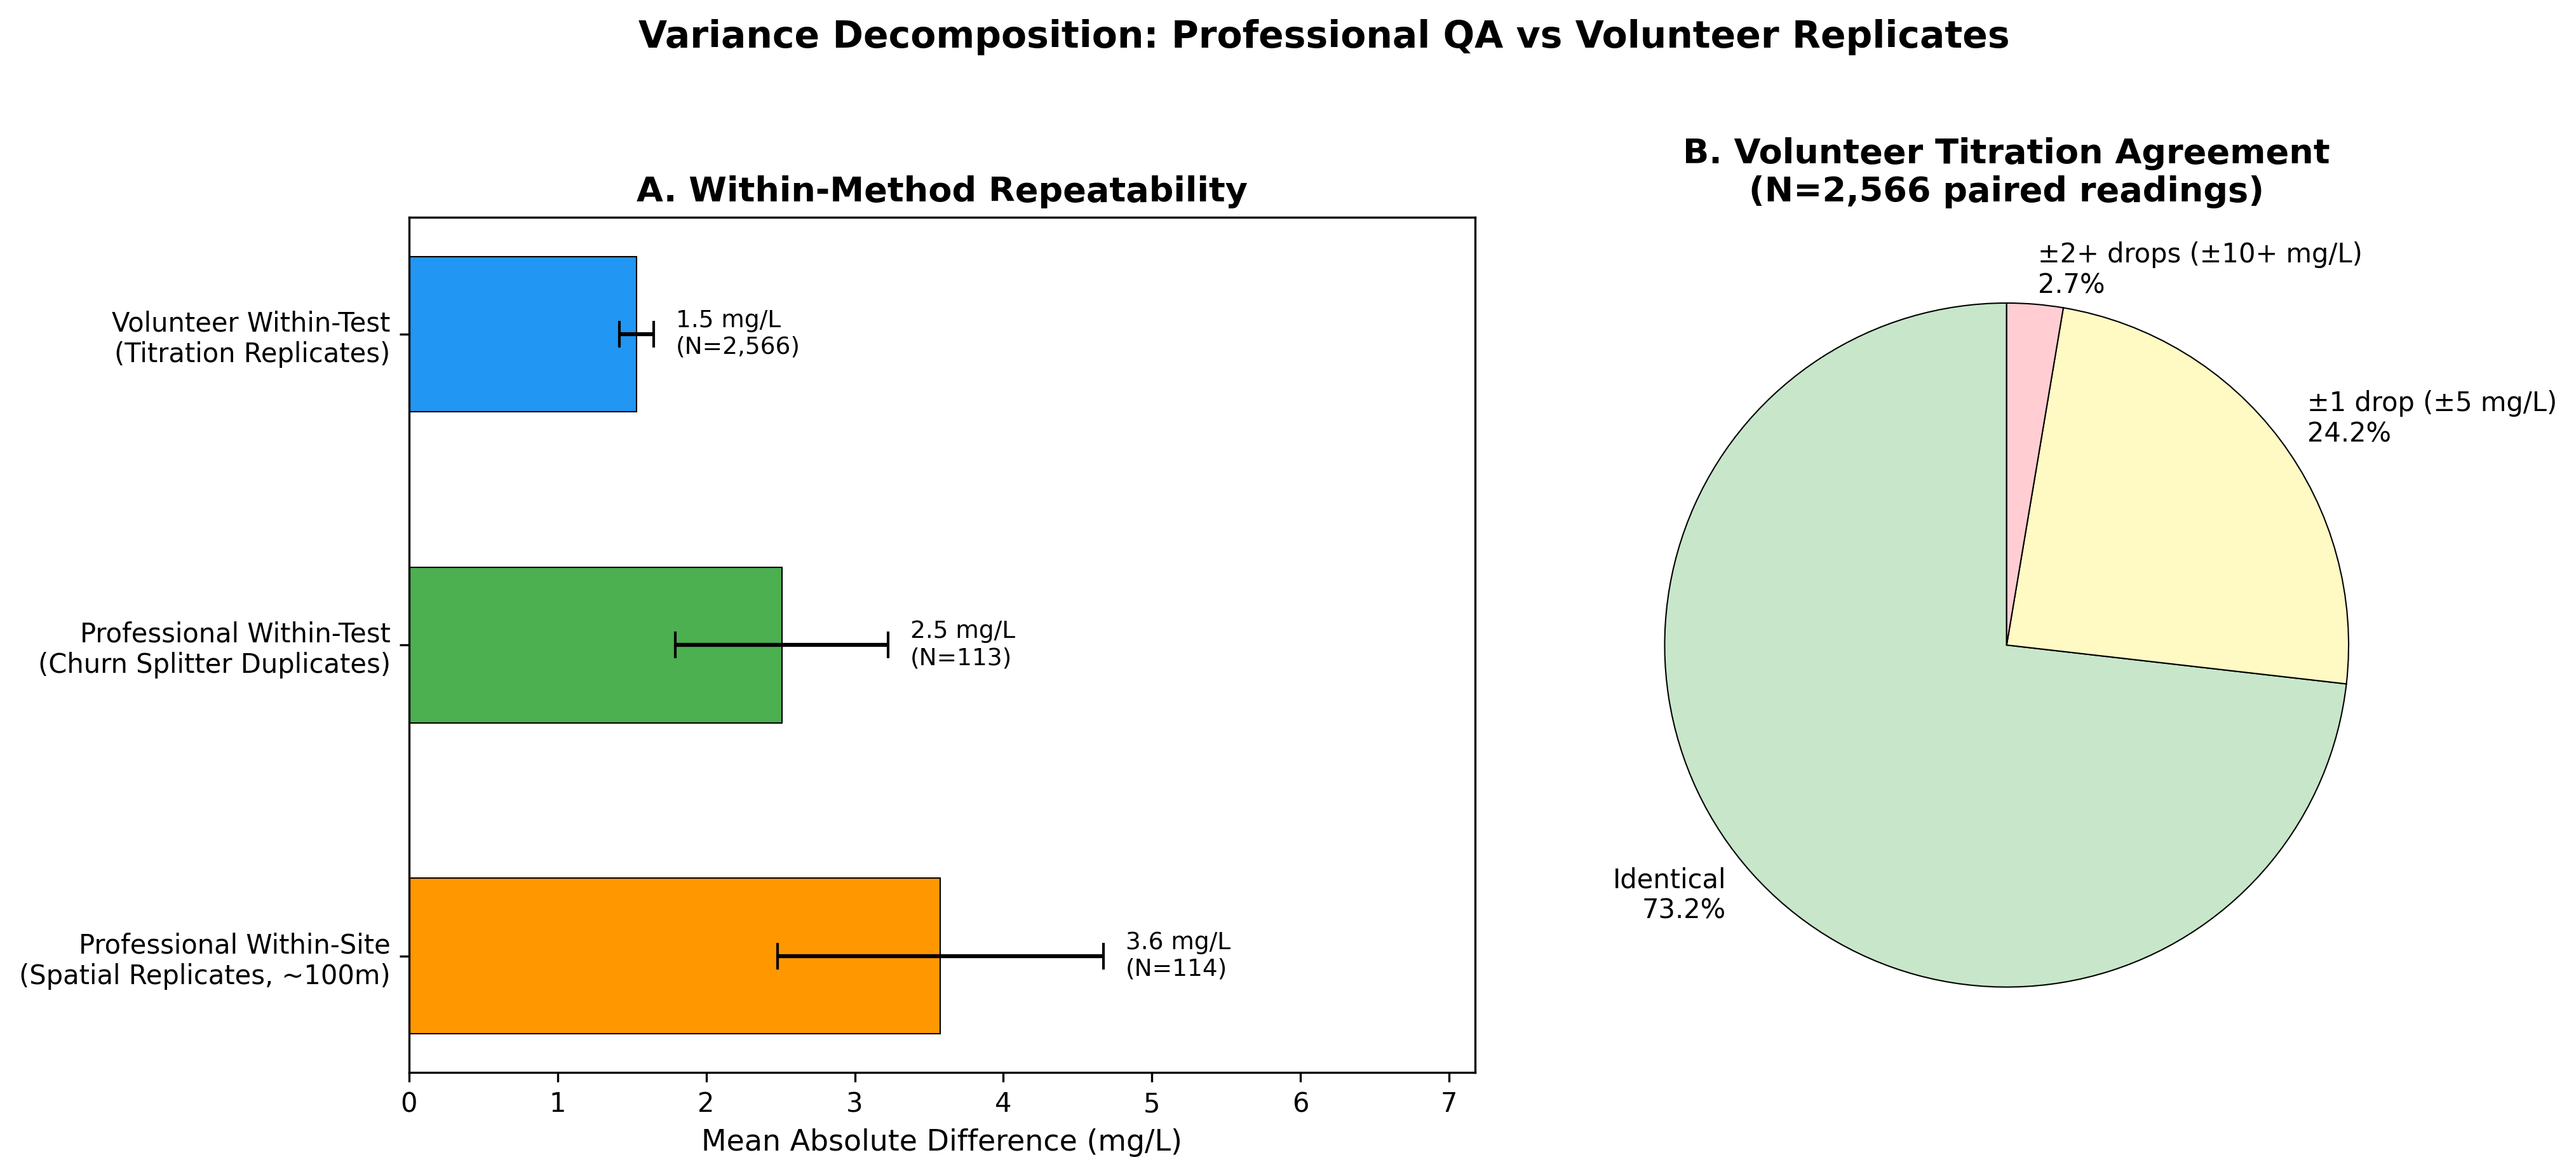
\includegraphics[width=\textwidth]{../data/outputs/phase2_lme/variance_decomposition.png}
\caption{Variance decomposition: professional QA vs.\ volunteer replicates. (A) Mean absolute difference (mg/L) with 95\% CI error bars for three measurement scenarios: volunteer within-test titration replicates ($N=2{,}566$, mean $|\mathrm{diff}| = 1.53$~mg/L), professional within-test churn splitter duplicates ($N=113$, mean $|\mathrm{diff}| = 2.51$~mg/L), and professional within-site spatial replicates $\sim$100~m apart ($N=114$, mean $|\mathrm{diff}| = 3.58$~mg/L). (B) Pie chart showing volunteer titration replicate agreement: 73.2\% identical, 24.1\% differ by one drop (5~mg/L), 2.7\% differ by two or more drops. 97.3\% of pairs agree within one drop.}
\label{fig:variance}
\end{figure}

\begin{figure}[p]
\centering
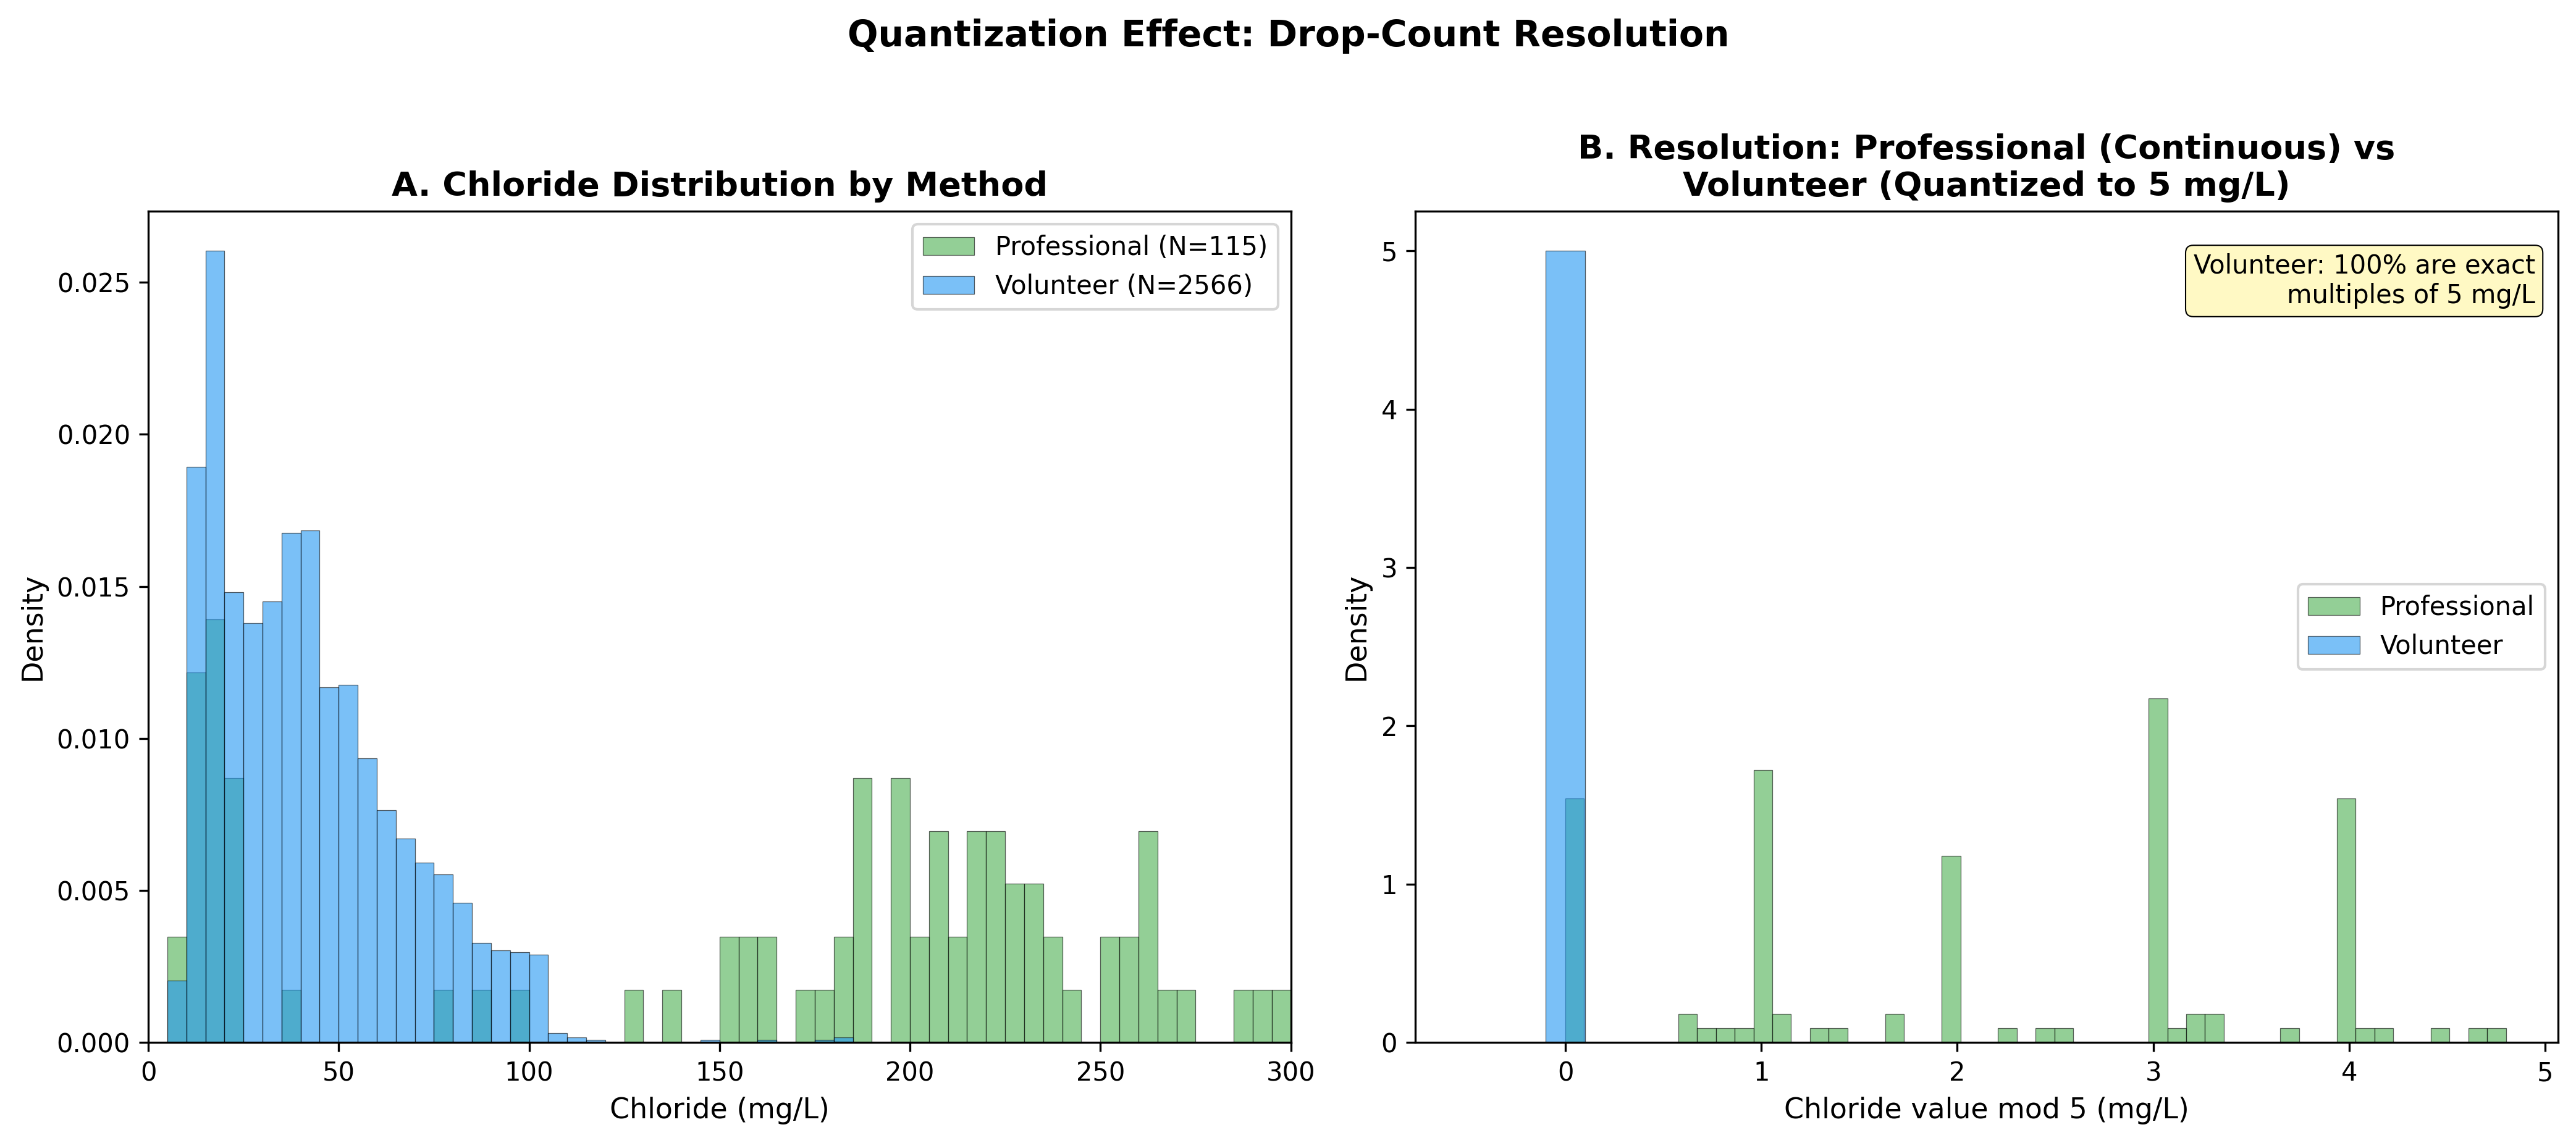
\includegraphics[width=\textwidth]{../data/outputs/phase2_lme/quantization_effect.png}
\caption{Quantization effect: drop-count resolution. (A) Histogram comparing the distribution of chloride values measured by professional instruments (smooth continuous distribution) and volunteer drop-count titration (discrete spikes at exact multiples of 5~mg/L). 100\% of volunteer readings are quantized to 5~mg/L intervals. (B) Resolution comparison confirming the discrete nature of volunteer measurements.}
\label{fig:quantization}
\end{figure}

\begin{figure}[p]
\centering
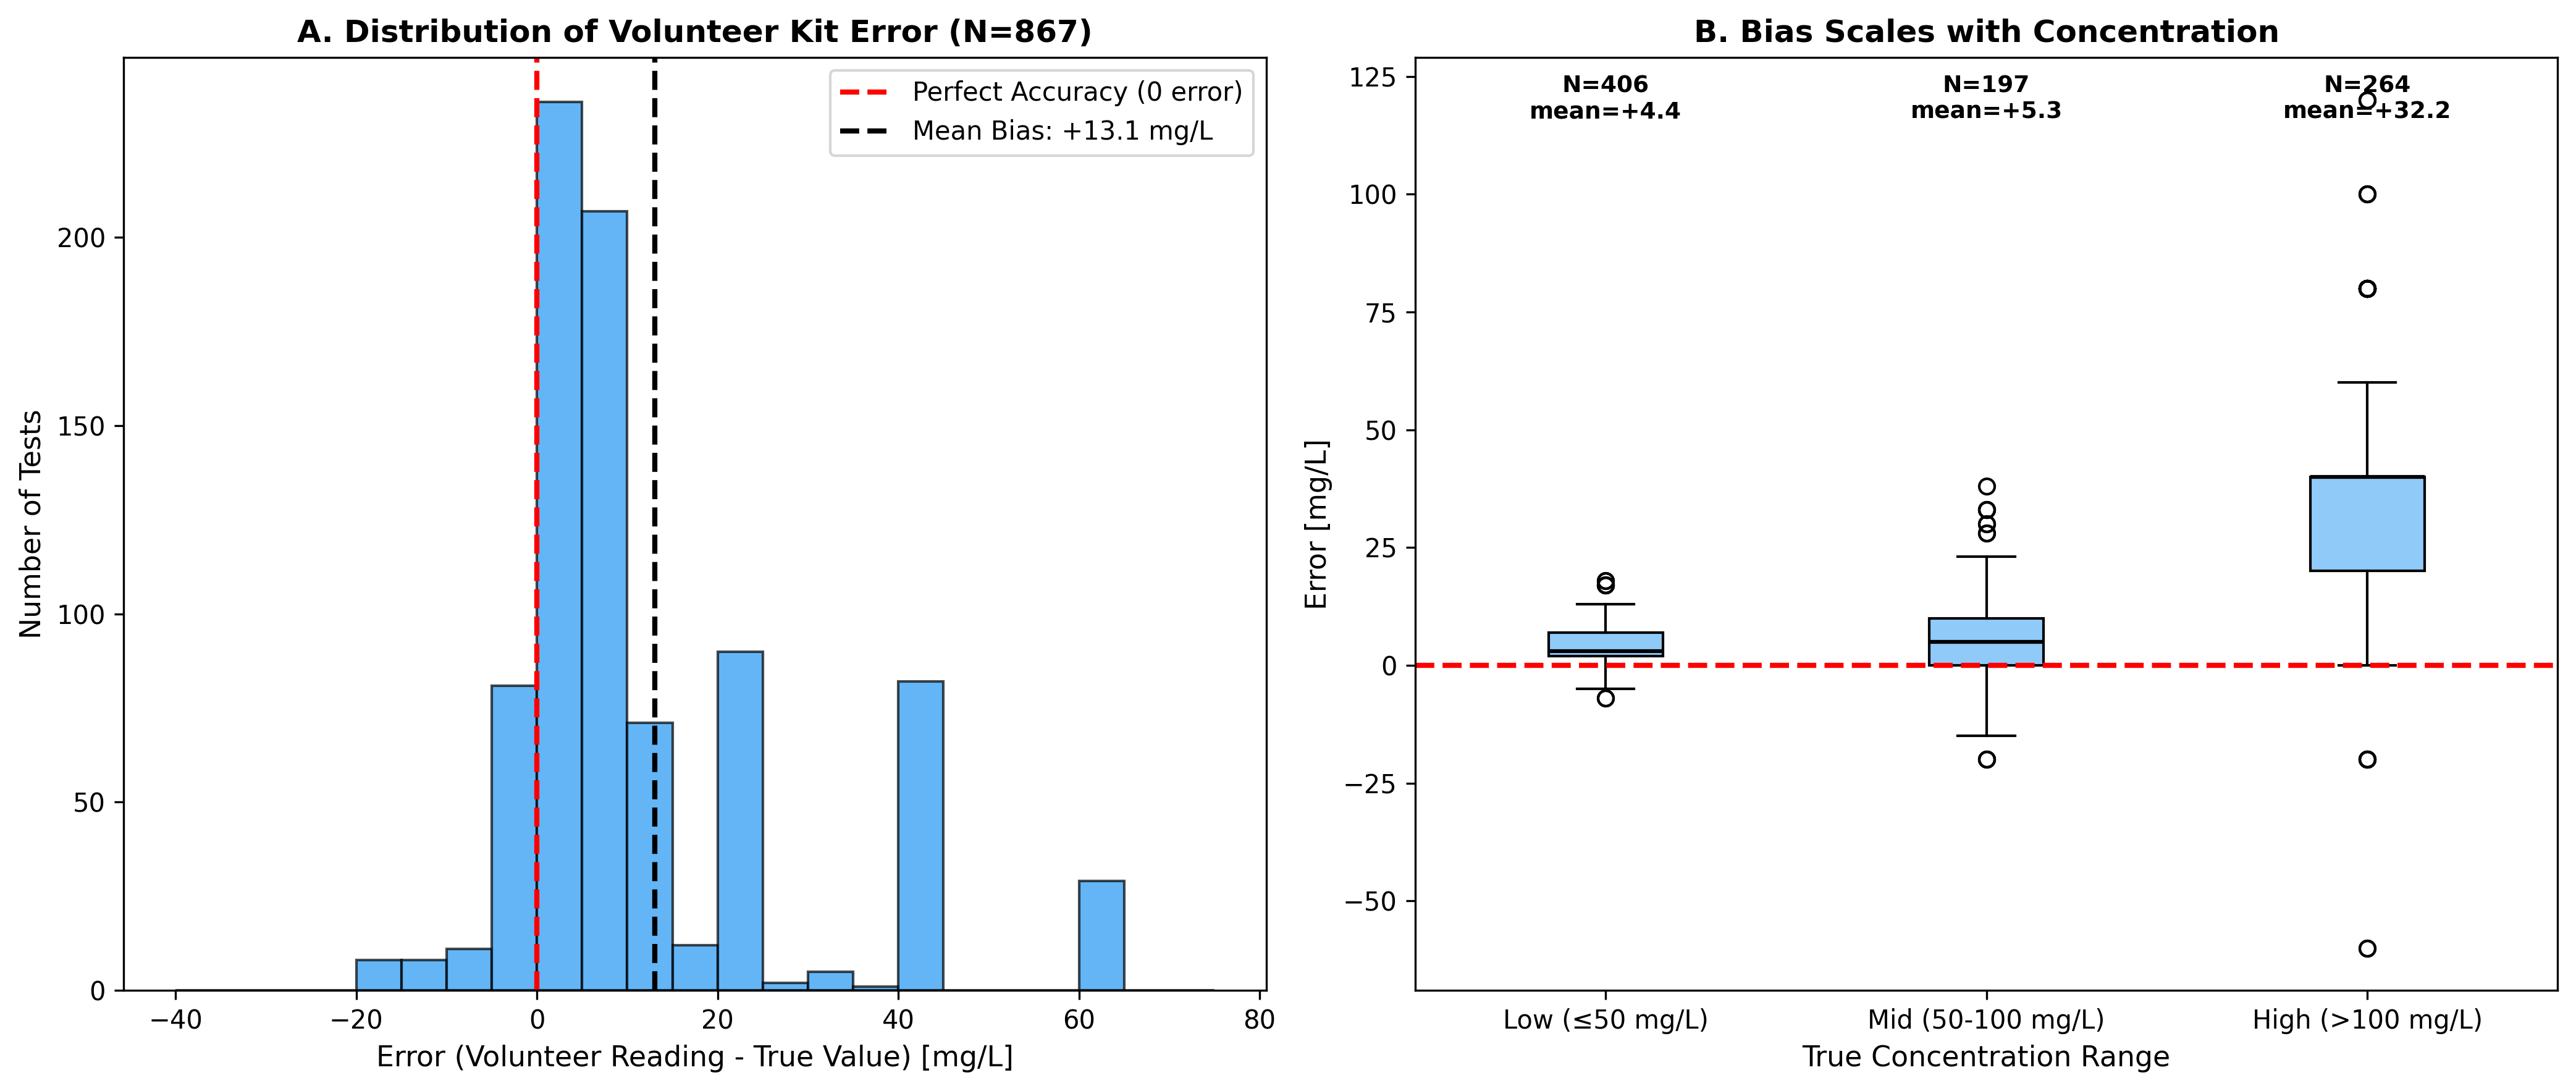
\includegraphics[width=\textwidth]{../data/outputs/phase2_lme/qa_accuracy_analysis.png}
\caption{Indoor QA accuracy analysis. (A) Histogram of volunteer kit error (volunteer reading $-$ known standard concentration, $N=867$ tests). The distribution is positively skewed, confirming systematic high bias. (B) Box plots of error stratified by concentration range, showing that bias scales with concentration: minimal at low concentrations ($\leq 50$~mg/L), moderate at mid-range (50--100~mg/L), and substantial at high concentrations ($> 100$~mg/L). Red dashed line at zero indicates perfect accuracy.}
\label{fig:qa}
\end{figure}

\begin{figure}[p]
\centering
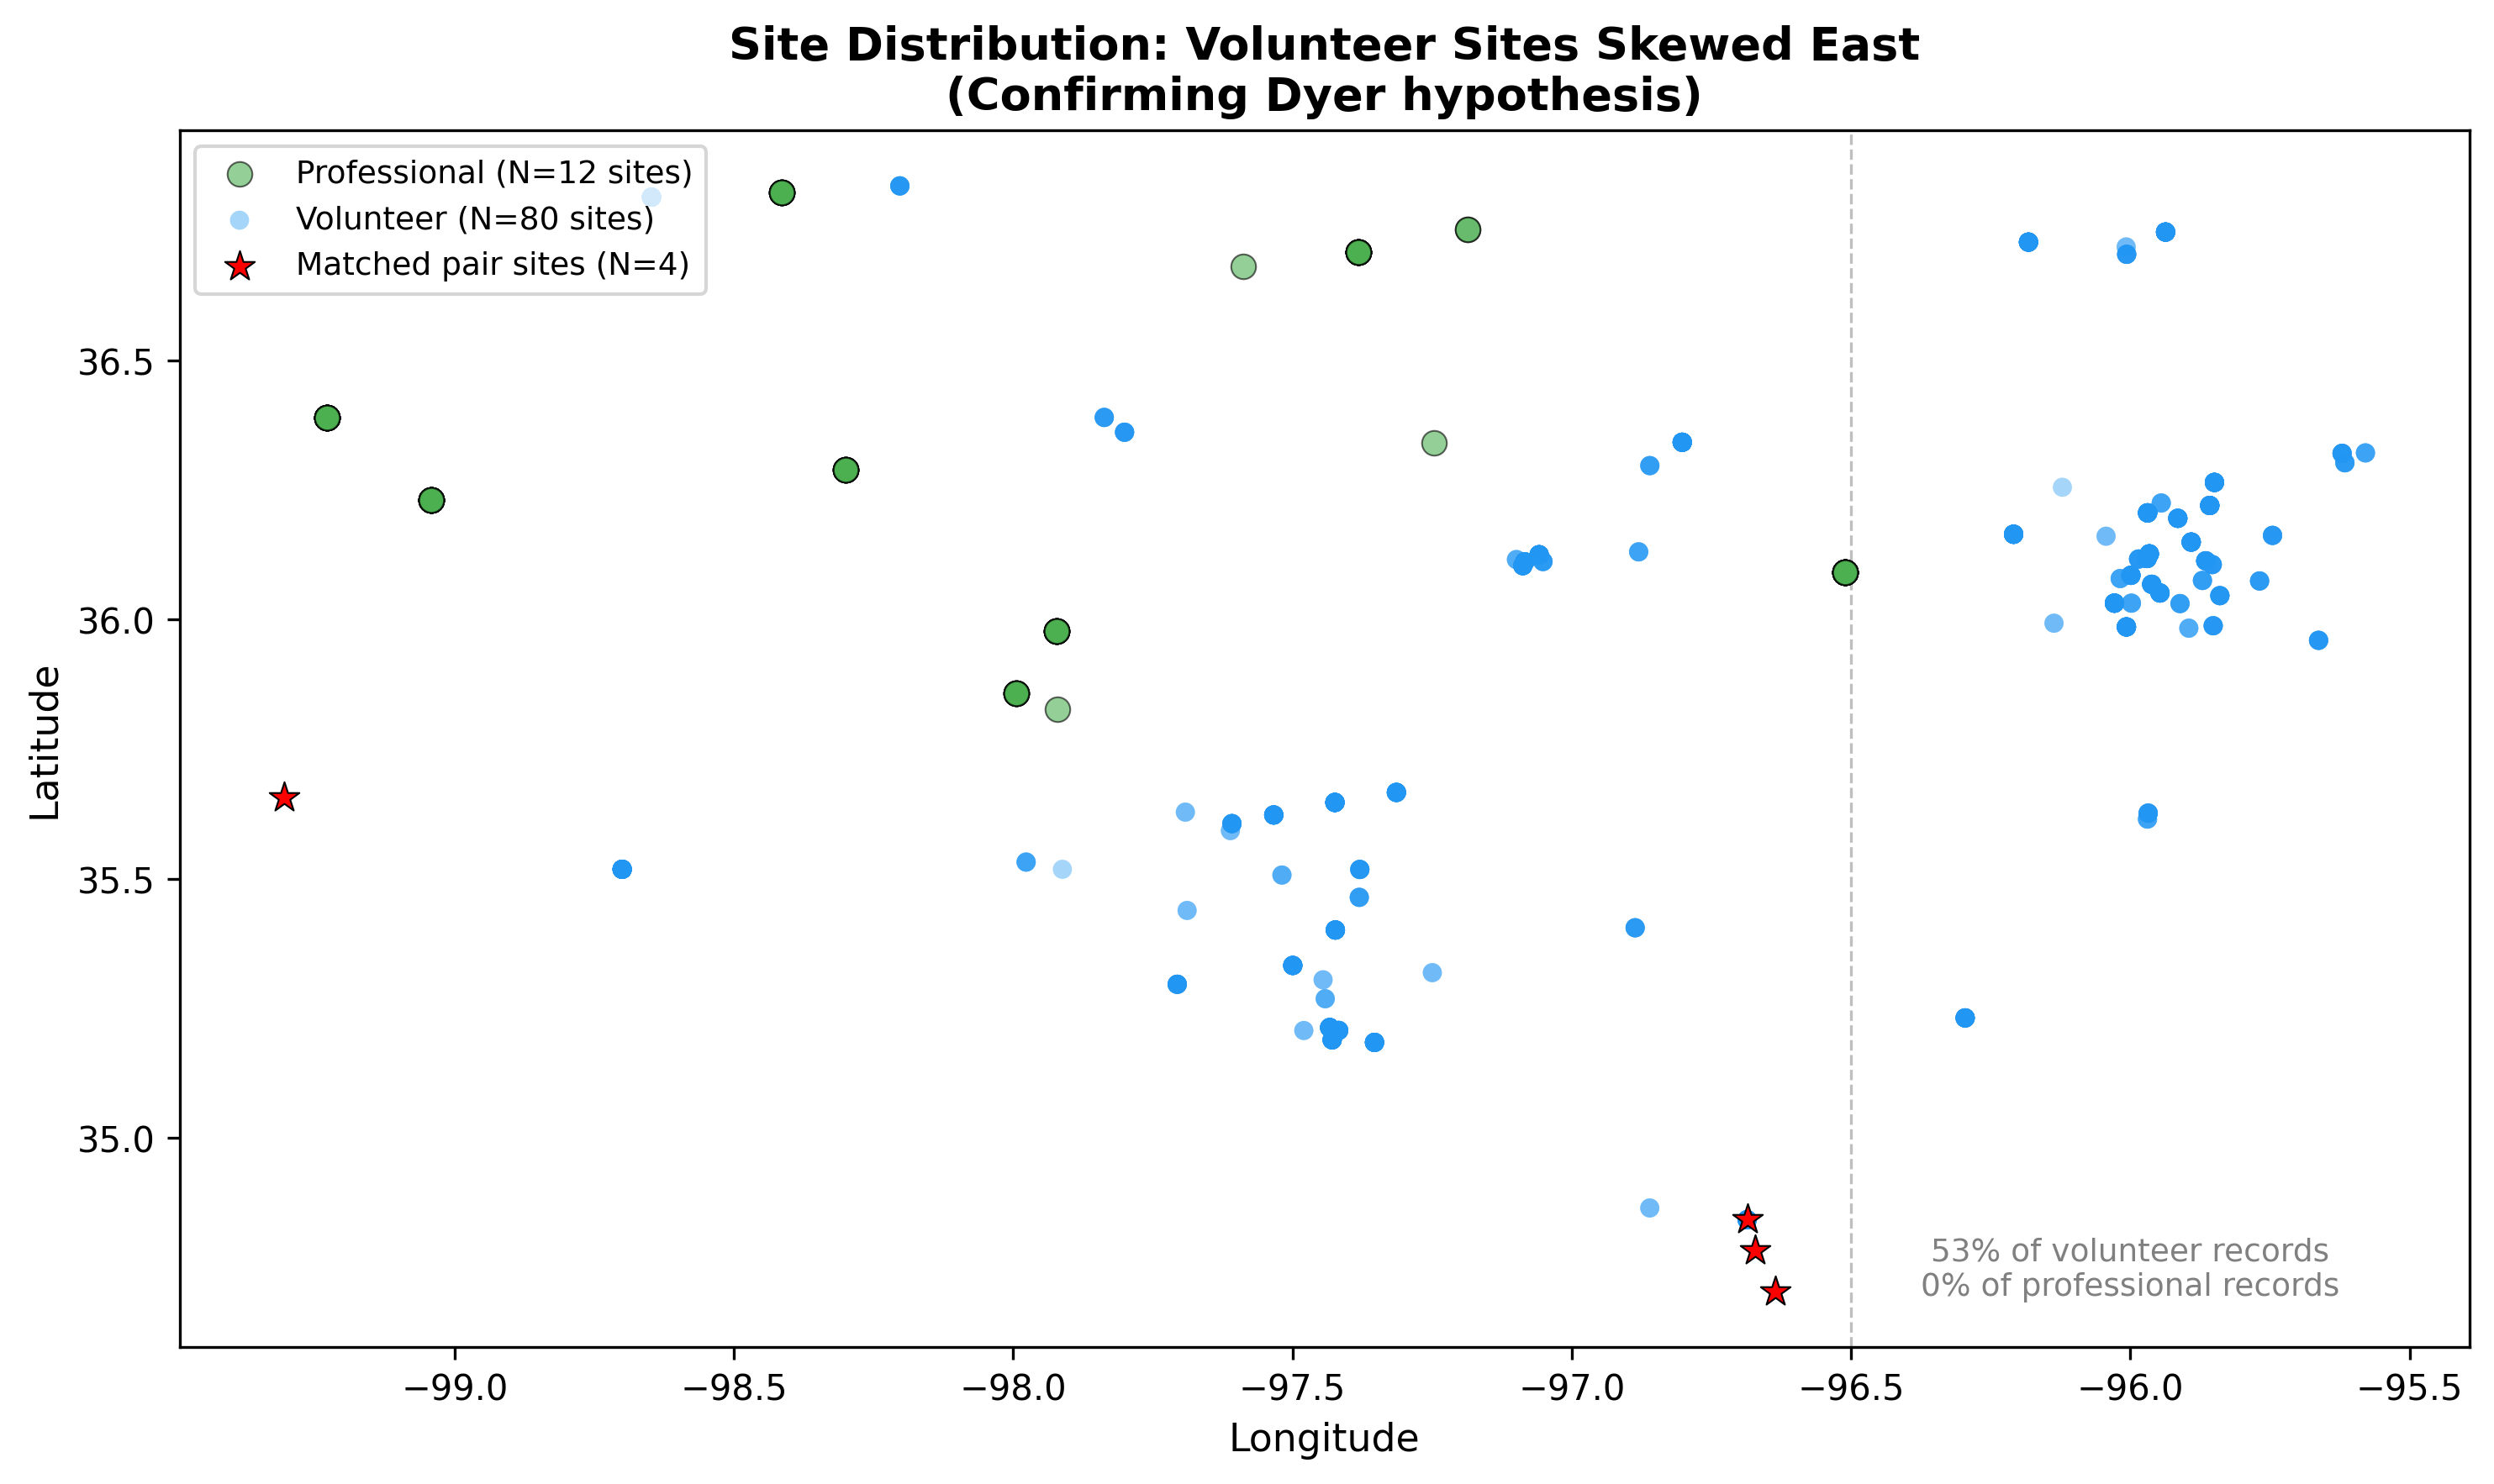
\includegraphics[width=\textwidth]{../data/outputs/phase2_lme/site_distribution_map.png}
\caption{Volunteer versus professional site distribution. Geographic distribution of professional sites (green, $N=12$) and volunteer sites (blue, $N=80$) within the QA dataset's spatiotemporal window. Volunteer sites are concentrated in eastern Oklahoma (mean longitude $-96.67^{\circ}$) while professional sites are distributed across central and western Oklahoma (mean longitude $-98.05^{\circ}$). The two groups have no geographic overlap along the gradient. The 1.4-degree East--West offset corresponds to approximately 115~km and aligns with the West--East salinity gradient documented by \citet{Dyer2025}, the source of the apparent observer bias in the regional model.}
\label{fig:sitemap}
\end{figure}

\begin{figure}[p]
\centering
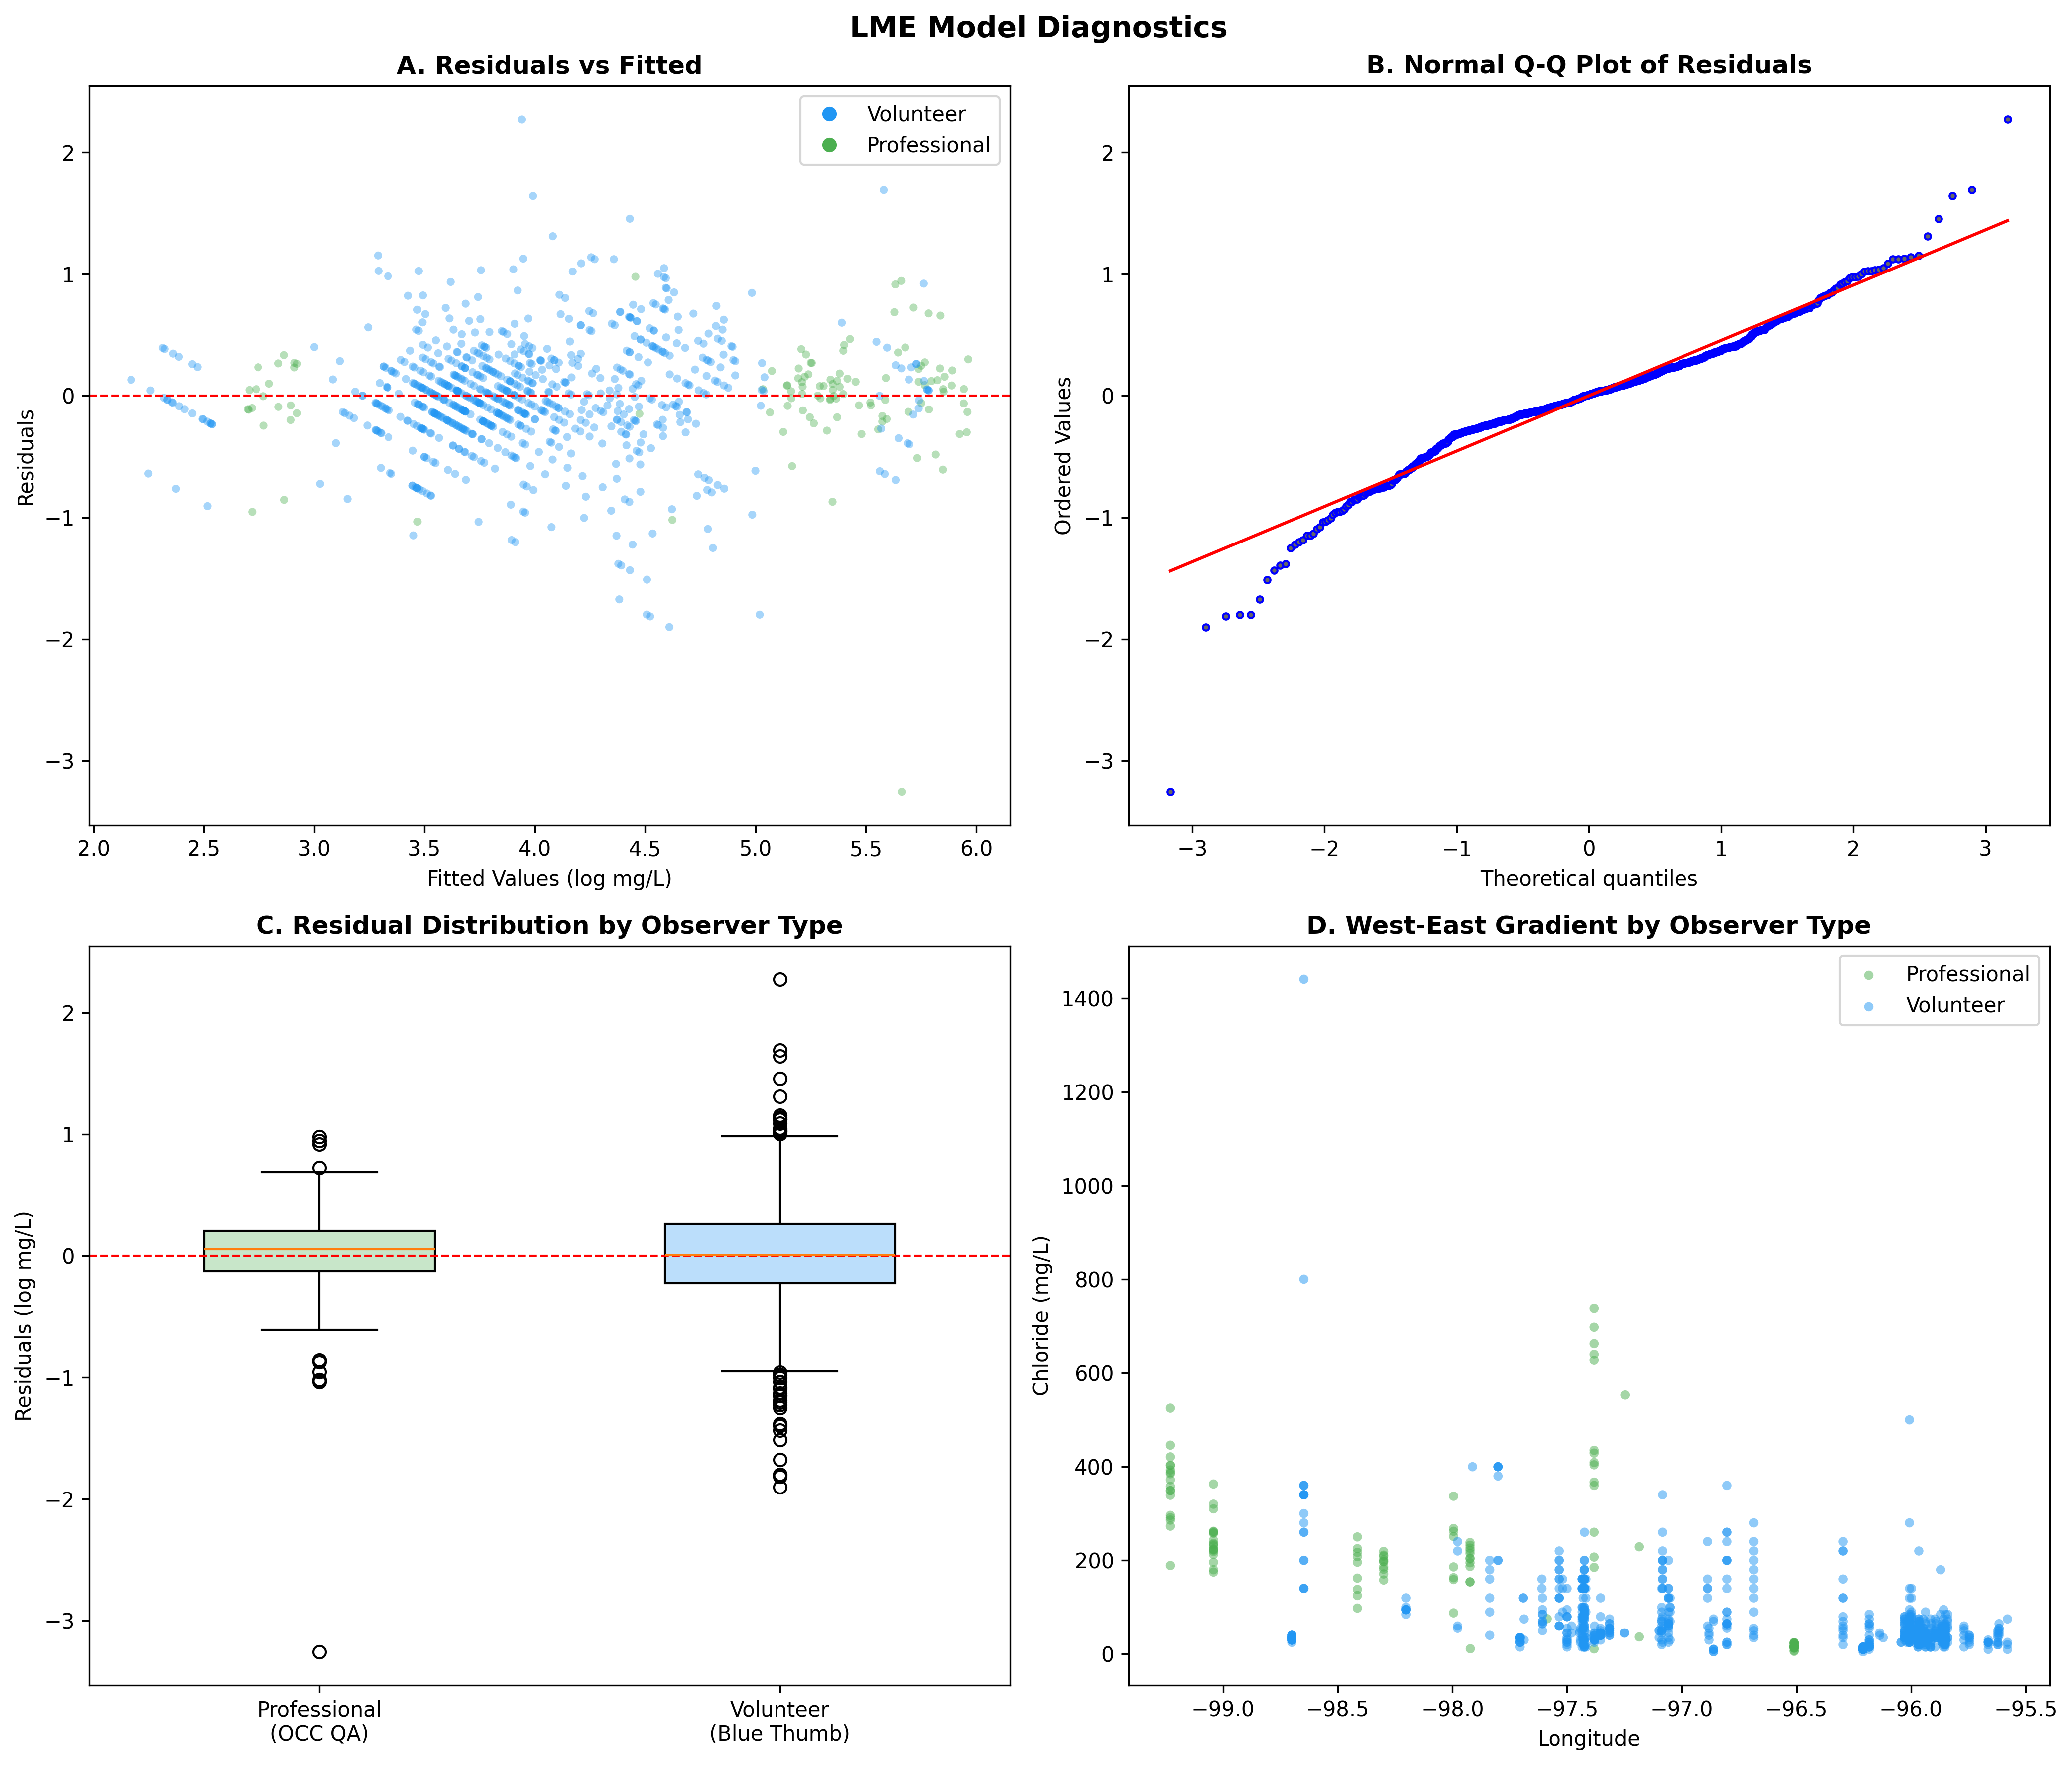
\includegraphics[width=\textwidth]{../data/outputs/phase2_lme/lme_diagnostics.png}
\caption{LME model diagnostics. (A) Residuals vs.\ fitted values, showing random scatter around zero with minor heteroscedasticity. (B) Normal Q--Q plot of residuals, indicating approximate normality with slight tail deviation. (C) Residual distributions by observer type (professional vs.\ volunteer), showing comparable spread. (D) Residuals by longitude, confirming the model adequately accounts for the West--East spatial gradient.}
\label{fig:diagnostics}
\end{figure}

\begin{figure}[p]
\centering
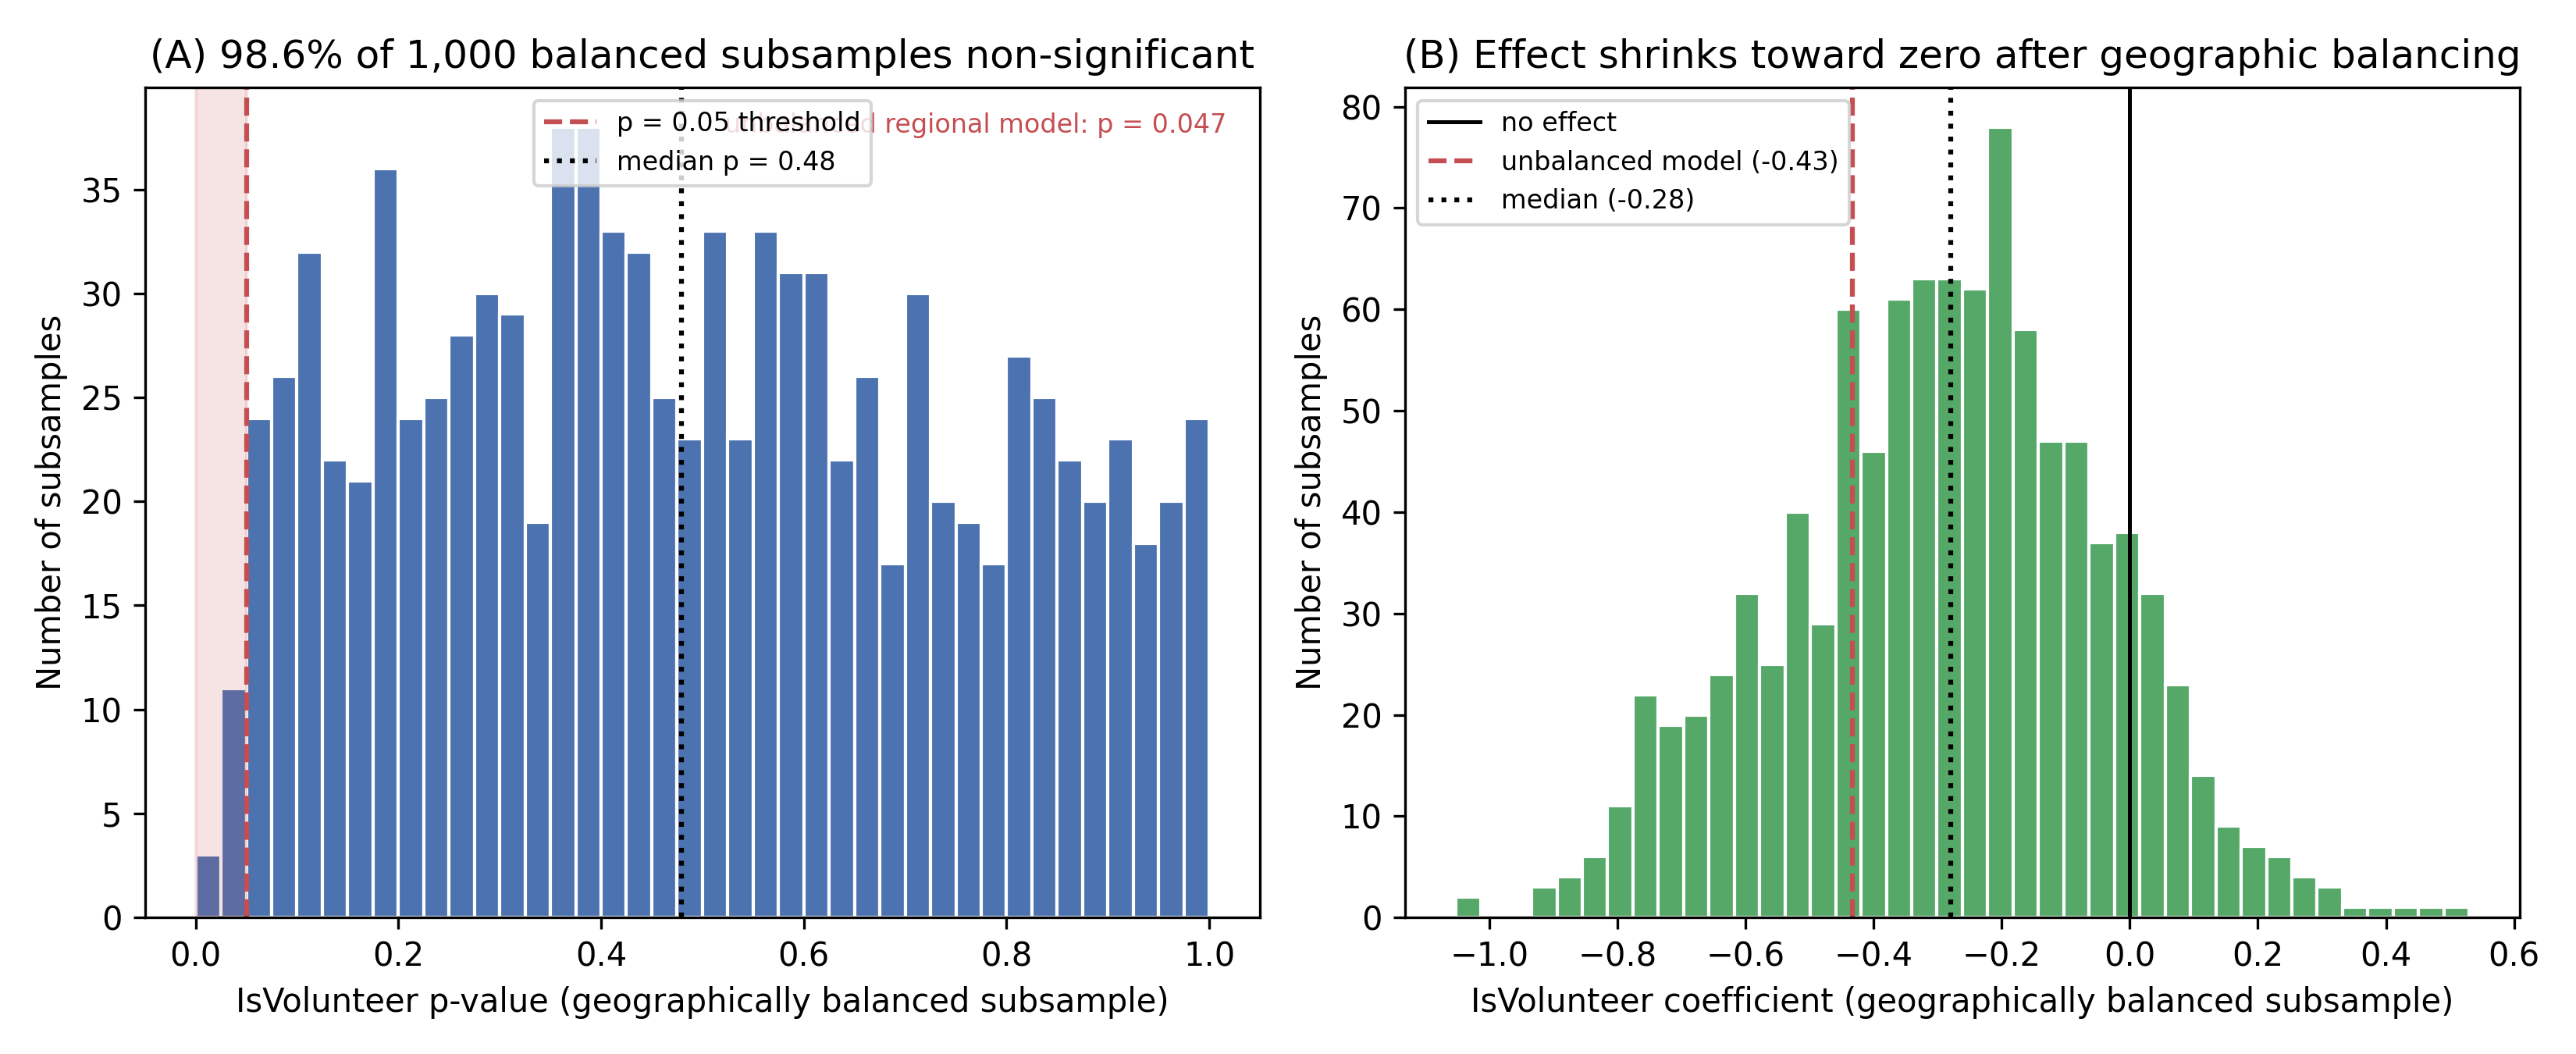
\includegraphics[width=\textwidth]{../data/outputs/phase2_lme/primary_result_subsampling.png}
\caption{Geographic confound test (primary result). (A) Distribution of the IsVolunteer $p$-value across 1{,}000 geographically balanced subsamples (12 volunteer sites, 3 per longitude quartile, matched to the 12 professional sites; fixed seed). The full regional model on the unbalanced data is significant ($p = 0.047$; the dashed line marks the 0.05 threshold), but after balancing the West--East gradient the volunteer effect is non-significant in 98.6\% of subsamples (median $p = 0.48$). (B) Distribution of the IsVolunteer coefficient across the same subsamples (median $-0.28$); the unbalanced regional estimate ($-0.433$) is shown for reference. The apparent observer bias is an artifact of monitoring-site geography, not observer error.}
\label{fig:subsampling}
\end{figure}

\begin{figure}[p]
\centering
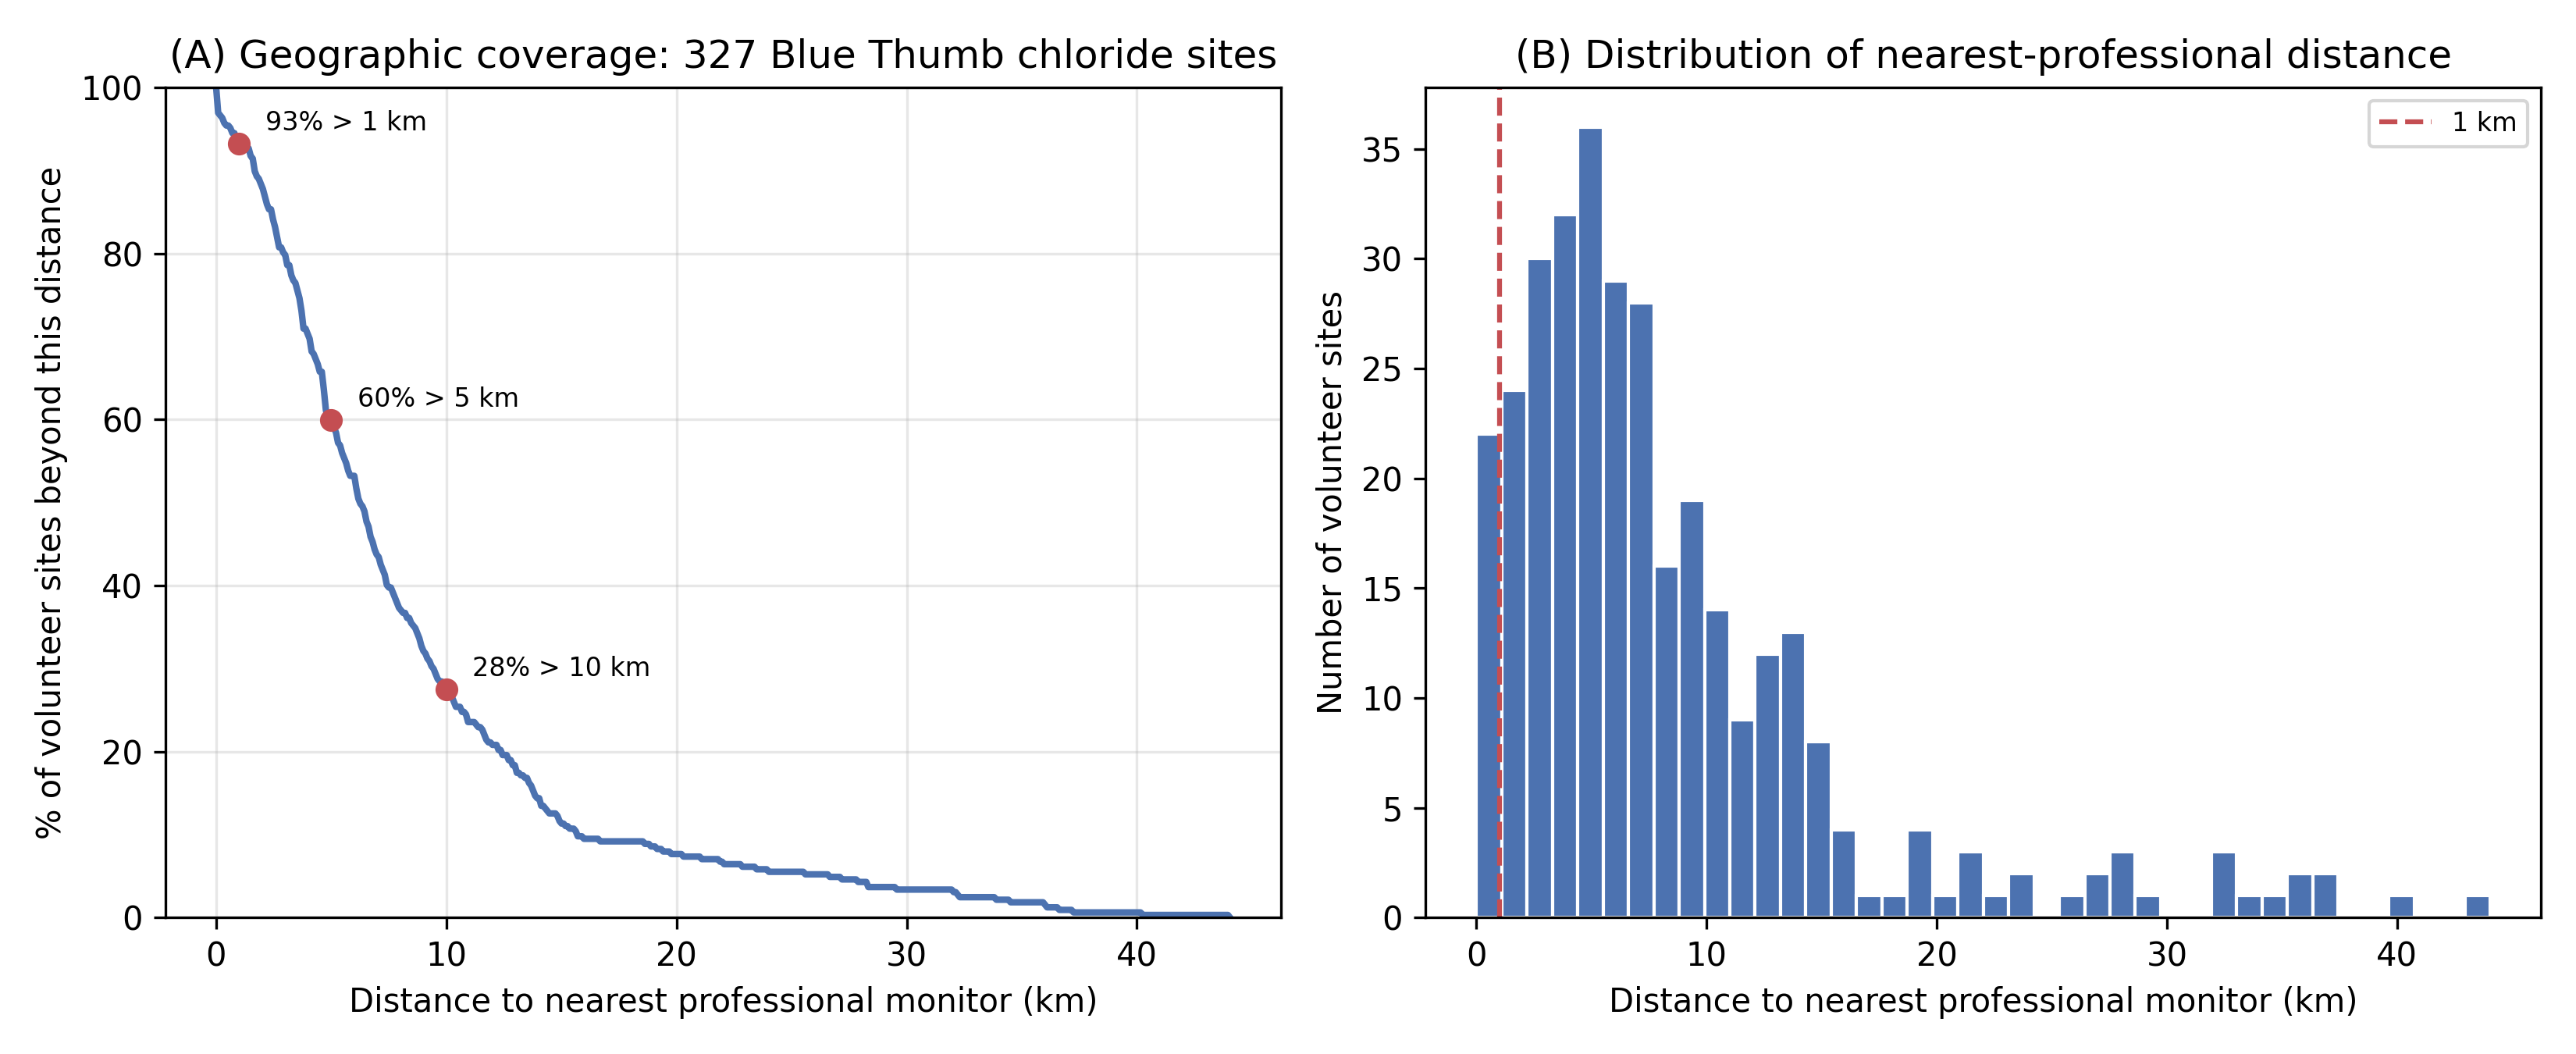
\includegraphics[width=\textwidth]{../data/outputs/phase2_lme/coverage_curve.png}
\caption{Geographic coverage of the Blue Thumb network. (A) Percentage of the 327 volunteer chloride monitoring sites whose nearest professional station (Haversine distance) exceeds a given distance: 93\% beyond 1~km, 60\% beyond 5~km, and 28\% beyond 10~km. (B) Distribution of the nearest-professional distance across all 327 sites. For the great majority of these stream reaches the volunteer record is the only record that exists.}
\label{fig:coverage}
\end{figure}

%%%%%%%%%%%%%%%%%%%%%%%%%%%%%%%%%%%%%%%%%%%%%%%%%%%%%%%%%%%%%
% Supplemental Information
%%%%%%%%%%%%%%%%%%%%%%%%%%%%%%%%%%%%%%%%%%%%%%%%%%%%%%%%%%%%%

\section*{Supplemental Information}

\subsection*{S1. Data preparation pipeline}

Full ETL pipeline description including: EPA WQP API query parameters, volunteer CSV normalization steps (WBID mapping, time parsing, coordinate coercion), data identity safeguards (\texttt{OKCONCOM\_WQX} exclusion from the volunteer dataset, SHA-256 enforcement), and complete configuration file documentation.

\subsection*{S2. Full statistical output tables}

Full mixed-effects fixed-effects and random-effects tables for the regional model ($N=895$, 92 sites) and for the geographically balanced subsample. Variance-decomposition summary statistics for all measurement types and the indoor QA error tables by concentration tier.

\subsection*{S3. Stratified subsampling balance check}

Longitude and chloride distributions for the full and geographically balanced datasets, the per-quartile site selection, and the IsVolunteer coefficient and $p$-value for the balanced subsample ($\beta = -0.2435$, $p = 0.5434$).

\subsection*{S4. Data availability and reproducibility}

Repository URL, installation instructions, the Phase 2 analysis entry points, and reproducibility manifest format. SHA-256 hashes for all input data files.

\end{document}
